已经到了这本书的最后一个章节了!我们学习了C++应用程序开发的基础知识,并讨论了架构和设计实际的应用程序。我们还深入研究了数据结构和算法,这是高效编程的核心。现在是时候利用所有这些技能来设计复杂的软件了——搜索引擎。 \par
随着互联网的普及,搜索引擎已经成为最受欢迎的产品。大多数用户通过搜索引擎开始他们的网络旅程。各种Web搜索服务,如谷歌、百度、Yandex等,接收大量的流量,每天服务数万亿的请求。搜索引擎处理每个请求的时间不到一秒。尽管它们维护了数千台服务器来处理负载,但它们高效处理的核心是数据结构和算法、数据架构策略和缓存。 \par
设计一个高效的搜索系统的问题不仅仅出现在网络搜索引擎中。本地数据库、客户关系管理(CRM)系统、会计软件等都需要健壮的搜索功能。在本章中,我们将发现搜索引擎的基本原理,并讨论用于构建快速搜索引擎的算法和数据结构。您将了解Web搜索引擎通常如何工作,并满足在需要高处理能力的项目中使用的新数据结构。你也将建立建立自己的搜索引擎,与现有大佬们竞争。 \par

本章中,我们将了解以下内容: \par

\begin{itemize}
	\item 了解搜索引擎的结构
	\item 理解并设计用于将关键字映射到搜索引擎中的反向索引
	\item 为搜索平台的用户设计和构建一个推荐引擎
	\item 利用知识图谱设计一个基于对话框的搜索引擎
\end{itemize}

\noindent\textbf{}\ \par
\textbf{编译器要求} \ \par
g++编译器需要添加编译选项 \texttt{-std=c++2a} 来编译本章的代码。可以从这里获取本章的源码件:https:/​/github.​com/PacktPublishing/Expert-CPP \par

\noindent\textbf{}\ \par
\textbf{了解搜索引擎的结构} \ \par
想象一下,世界上有数十亿个网页。在搜索引擎界面中输入一个单词或短语,不到一秒钟就会返回一长串搜索结果。搜索引擎处理这么多网页的速度是不可思议的。它怎么能这么快找到正确的文档?为了回答这个问题,我们将做一个程序员能做的最明智的事情,设计一个我们自己的引擎。 \par
下图展示了搜索引擎背后的基本思想: \par

\begin{center}
	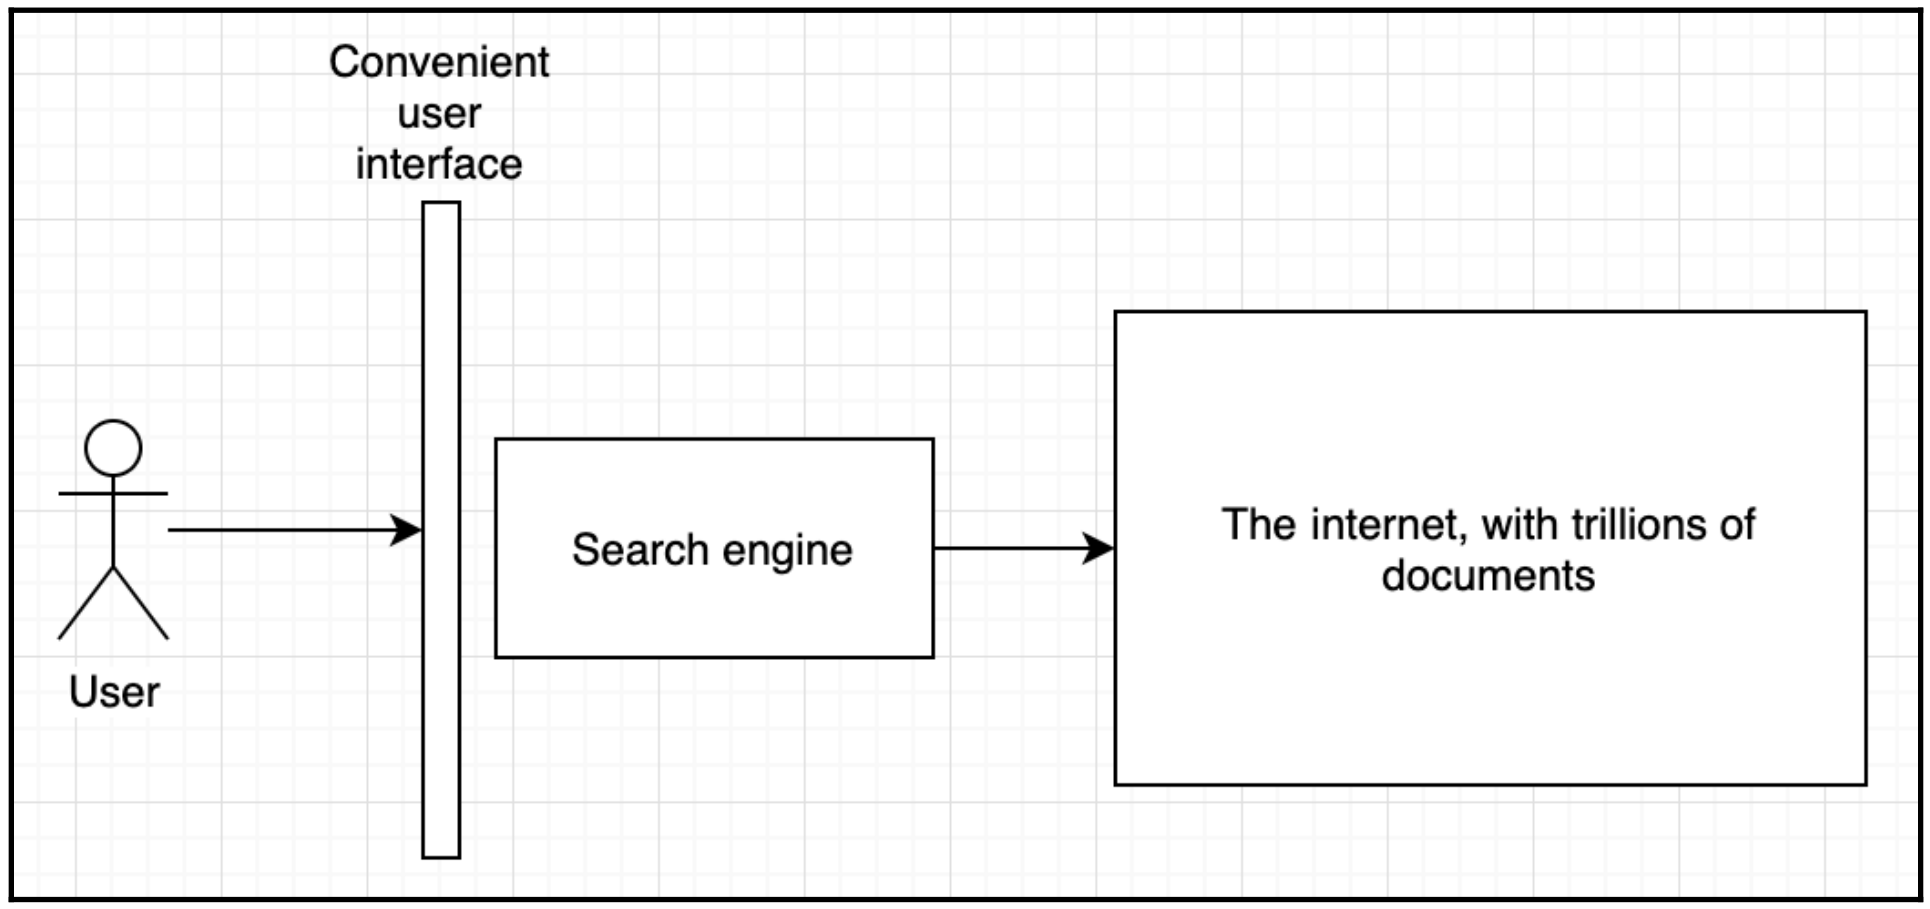
\includegraphics[width=0.8\textwidth]{content/Section-3/Chapter-16/1}
\end{center}

用户使用搜索引擎的用户界面输入单词。搜索引擎扫描所有文档,筛选它们,根据相关性对它们进行排序,并尽可能快地响应用户。我们的主要兴趣在于Web搜索引擎的实现。要想找到某样东西,就需要在数十亿份文件中搜索。 \par
让我们尝试设计一种方法来从数十亿的文档中(为了简洁起见,我们将Web页面称为文档)找到\texttt{Hello,world!}。扫描每一份文件寻找这个短语会花费大量的时间。如果我们认为每个文档至少有500个单词,那么搜索一个特定的单词或单词的组合将花费大量时间。事先扫描所有文件会更实际些。这个扫描过程包括为文档中出现的每个单词建立索引,并将信息存储在数据库中,这也称为索引文档。当用户输入一个短语时,搜索引擎将在其数据库中查找该词,并以满足查询的文档链接作出回应。 \par
搜索文档之前,引擎应该验证用户的输入。用户在短语中出现拼写错误并不罕见。除了拼写错误,如果引擎自动完成单词和短语,用户体验会更好。例如,当用户输入\texttt{hello}时,引擎可能会建议搜索短语\texttt{hello, world!}。一些搜索引擎跟踪用户,存储有关他们最近搜索的信息、他们用来发出请求的设备的详细信息等,例如:如果搜索引擎知道用户的操作系统,那么用户搜索如何重启计算机将得到更好的结果。如果是Linux发行版,搜索引擎将对搜索结果进行排序,使描述基于Linux的计算机重新启动的文档首先出现。 \par
我们还应该注意网络上经常出现的新文件。后台工作可能会不断地分析网络以找到新的内容,我们称这个工作为爬虫,因为它爬虫网络和索引文档。爬虫程序下载文档以解析其内容并构建索引。已经建立索引的文档可能会更新,甚至删除。因此,另一项后台工作应该负责定期更新现有文档。您可能会遇到术语“蜘蛛”,它表示在Web上搜索和解析文档的任务。 \par
下面的图表更详细地说明了搜索引擎的结构: \par

\begin{center}
	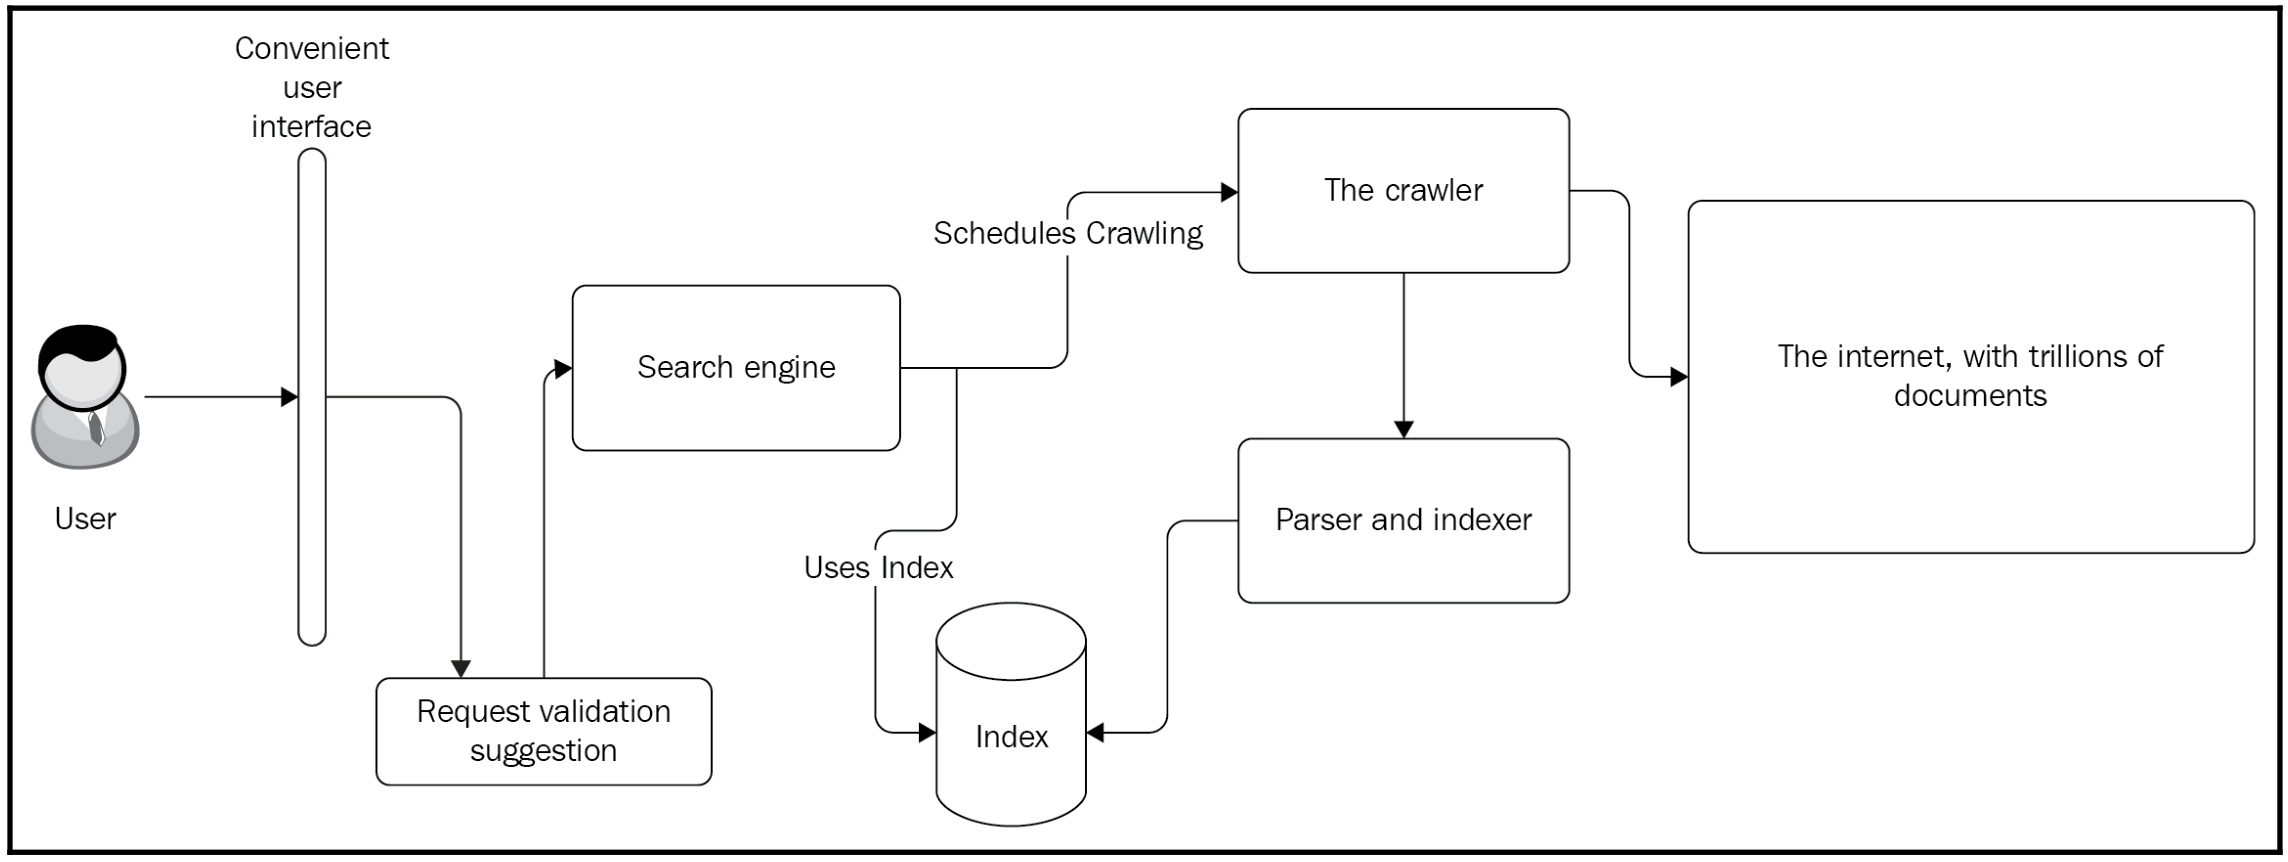
\includegraphics[width=1.0\textwidth]{content/Section-3/Chapter-16/2}
\end{center}

搜索应用广泛。想象一下最简单的搜索形式——在数组中查找单词: \par

\begin{lstlisting}[caption={}]
using words = std::vector<std::string>;
words list = get_list_of_words(); // suppose the function is implemented

auto find_in_words(const std::string& term)
{
	return std::find(list.begin(), list.end(), term);
}
\end{lstlisting}

虽然前面的例子适用于最简单的搜索引擎,但真正的问题是设计一个可伸缩的搜索引擎。我们不希望通过搜索字符串数组来满足用户请求。相反,应该努力实现一个可扩展的搜索引擎,能够搜索数百万个文档。这需要大量的思考和设计,因为从数据结构的正确选择到数据处理的高效算法,一切都很重要。现在让我们更详细地讨论搜索引擎的组件。我们将结合前面章节学到的所有技巧来设计一个好的搜索引擎。 \par

\noindent\textbf{}\ \par
\textbf{提供方便的用户界面} \ \par
投入时间和资源来构建一个细粒度的用户界面是至关重要的,它将提供惊人的用户体验。界面越简单,使用效果越好。我们将以占据市场主导地位的谷歌为例。它在页面中心有一个简单的输入字段。用户在字段中输入他们的请求,引擎会给出一些短语: \par

\begin{center}
	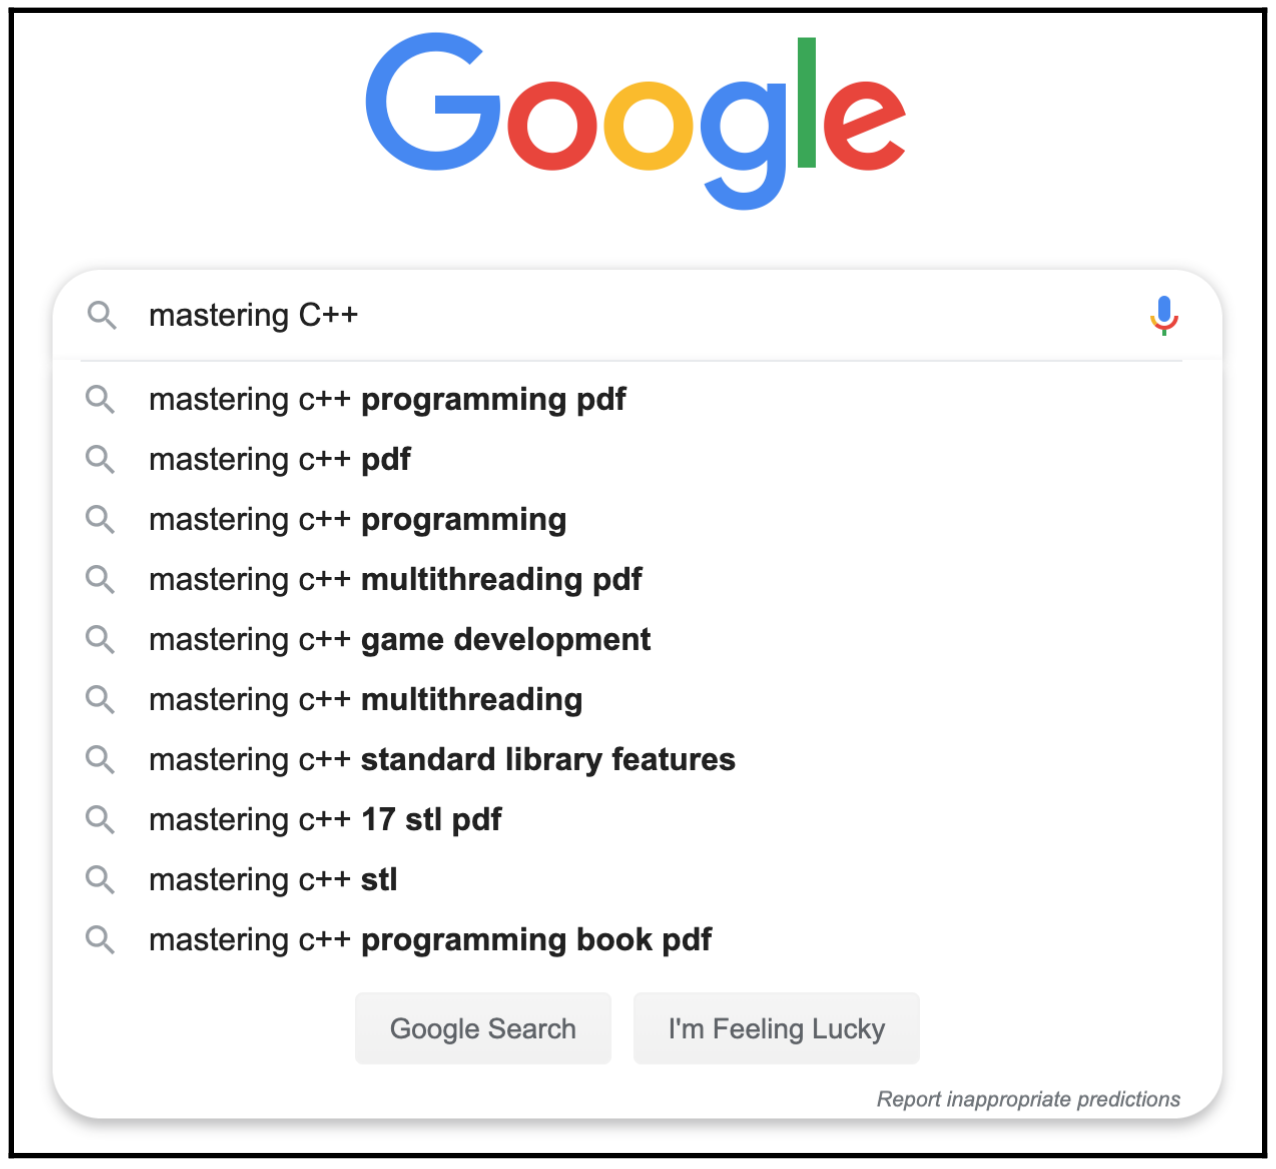
\includegraphics[width=0.8\textwidth]{content/Section-3/Chapter-16/3}
\end{center}

我们并不认为用户是懒惰的人,但是提供一个建议列表是很有帮助的,因为有时候用户并不知道他们想要的确切术语。让我们专注于建议列表的结构和实施。毕竟,我们感兴趣的是解决问题,而不是设计良好的用户界面。本章不讨论用户界面设计,而是专注于搜索引擎的后端。然而,在继续之前,还有一件事我们应该考虑,这里实现的搜索引擎是基于对话框的。用户查询引擎,并可以从几个答案中进行选择,以缩小结果列表。例如,假设用户查询一台计算机,搜索引擎询问一台台式机或笔记本电脑?这大大减少了搜索结果,为用户提供了更好的结果。我们将使用决策树来实现这一点。在此之前,让我们先了解一下搜索引擎的复杂性。 \par
首先是输入标记化的问题。这与文档解析和搜索短语分析有关。您可能会构建一个很好的查询解析器,它会因为用户在查询中犯了错误而中断。让我们看看处理模糊查询的两种方法。 \par

\noindent\textbf{}\ \par
\textbf{处理查询中的拼写错误} \ \par
用户在输入时出现拼写错误的情况并不少见。虽然这看起来是一件简单的事情,但对于搜索引擎设计者来说却是一个真正的问题。如果用户输入的是\texttt{helo world}而不是\texttt{hello world},那么搜索数百万个文档可能会出现意想不到的错误结果。您可能熟悉搜索引擎提供的自动建议,例如:当我们输入错误时,谷歌的搜索界面是这样的: \par

\begin{center}
	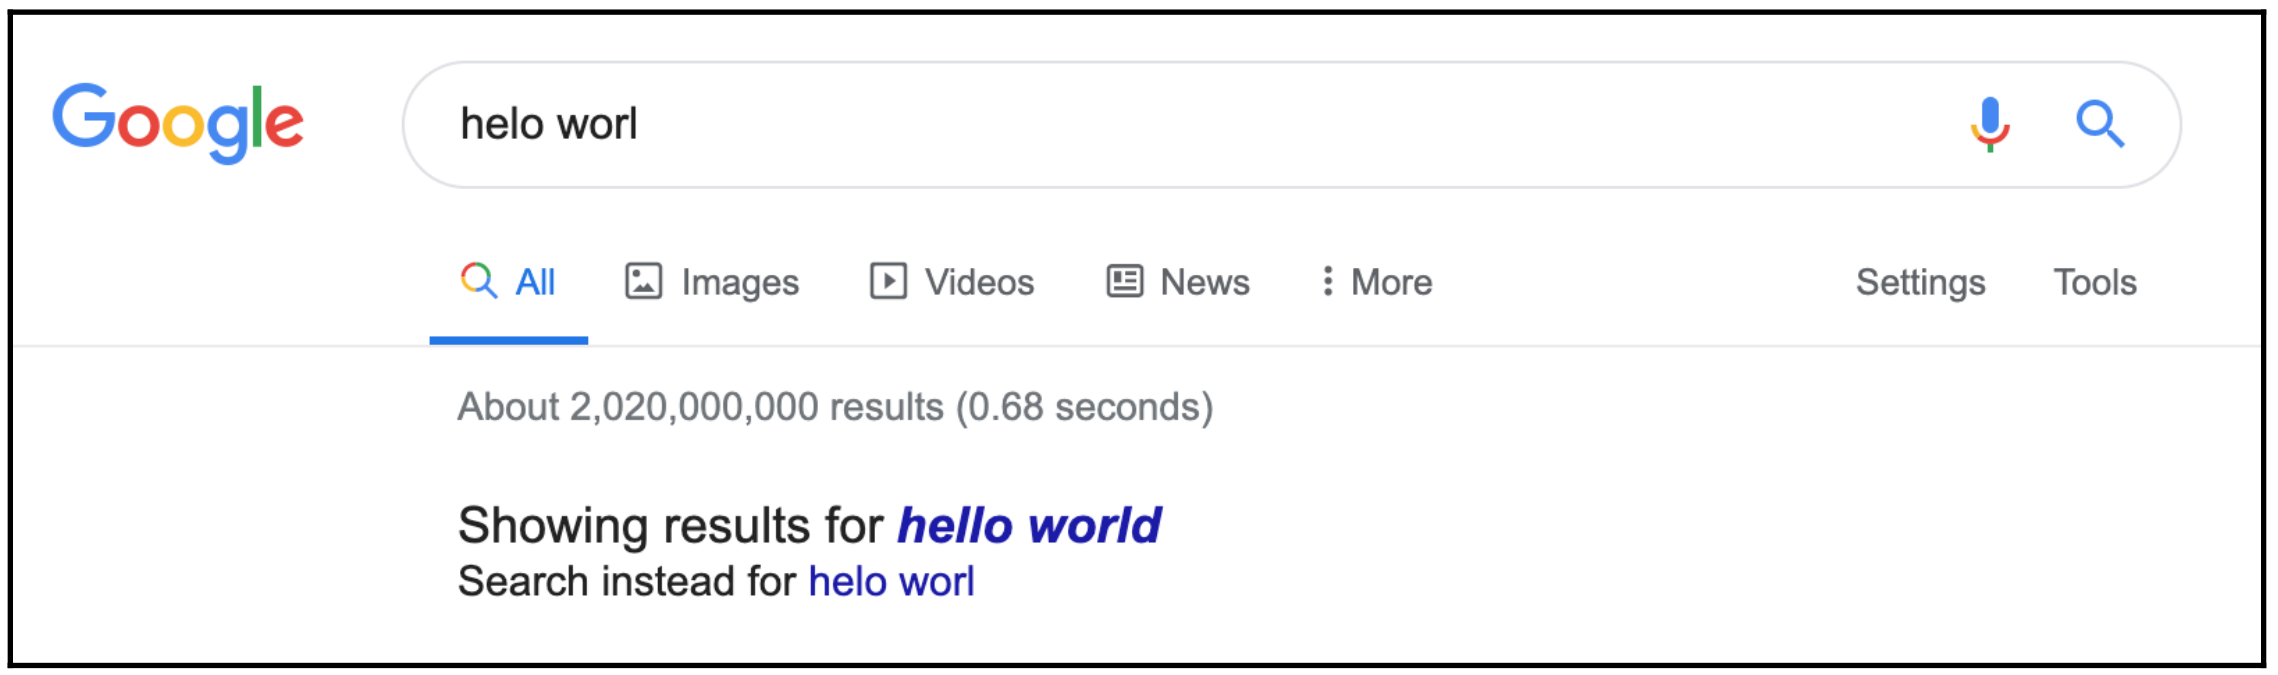
\includegraphics[width=1.0\textwidth]{content/Section-3/Chapter-16/4}
\end{center}

请注意截图底部的两行。其中之一是显示\texttt{hello world}的结果,这表明搜索引擎假设用户输入的查询有拼写错误,并主动显示正确的查询结果。然而,仍然有可能用户确实想要搜索他们输入的确切单词。因此,用户体验提供了下一行作为搜索\texttt{helo world}的结果。 \par
因此,在构建搜索引擎时,我们需要解决几个问题,首先是用户请求。首先,我们需要为用户提供一个简单的输入文本的界面。界面还应该与它们交互,以提供更好的结果,这包括基于部分输入的单词提供建议。使搜索引擎与用户交互是我们将在本章讨论的用户界面的另一个改进。 \par
接下来是检查拼写错误或不完整的单词,这不是一项容易的任务。在字典中保存所有单词的列表并比较用户输入的单词可能需要一段时间。为了解决这个问题,必须使用特定的数据结构和算法。例如,在检查用户查询中的拼写错误时,查找单词之间的Levenshtein距离可能会有帮助。Levenshtein距离是一个单词中应该添加、删除或替换的字符数,以使它等于另一个字符。例如,单词world和world之间的Levenshtein距离是1,因为从world中删除字母d或将字母d添加到world中会使这两个单词相等。单词编码和坐下之间的距离是4,因为以下四次编辑将一个单词变为另一个: \par

\begin{itemize}
	\item coding -> cod\textbf{t}ing (在中间插入t) 
	\item co\textbf{d}ting -> co\textbf{t}ting (用t替换d) 
	\item c\textbf{o}tting -> c\textbf{i}tting (用i替换o) 
	\item \textbf{c}itting -> \textbf{s}itting (用s替换c) 
\end{itemize}

如果我们将每个用户的输入与数万个单词进行比较,找出最接近的单词,那么处理过程将需要多长时间。另一种方法是使用一个大的try(数据结构)预先发现可能的拼写错误。一个try是一个有序的搜索树,其中键是字符串。下面的图表代表了一次尝试: \par

\begin{center}
	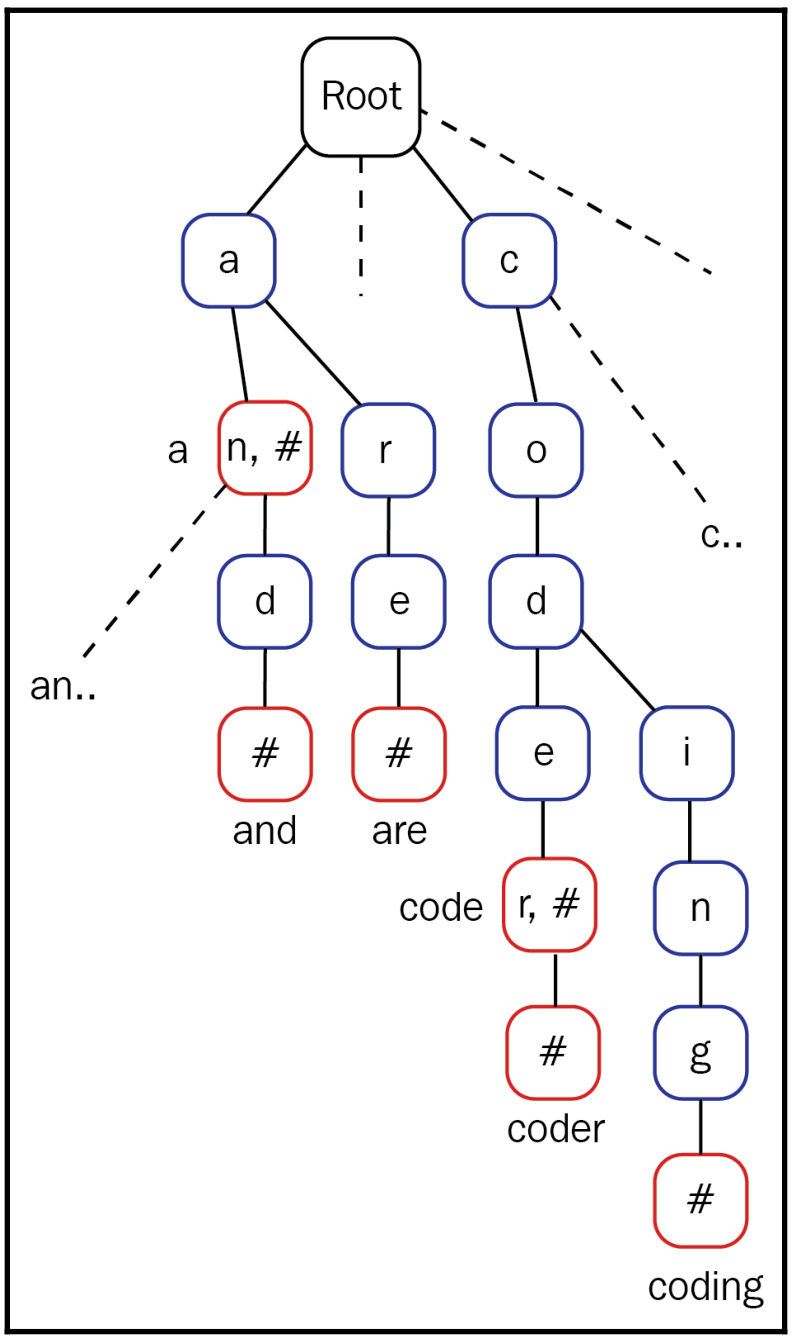
\includegraphics[width=0.6\textwidth]{content/Section-3/Chapter-16/5}
\end{center}

每个路径代表一个有效的字。例如,a节点指向n和r节点。注意n后面的\#。它告诉我们,到这个节点的路径代表一个单词an。但是,它继续指向d, d后面跟着另一个\#,这意味着到这个节点的路径表示另一个单词和。同样的逻辑也适用于其余的试验。例如,想象一下world这个单词的部分: \par

\begin{center}
	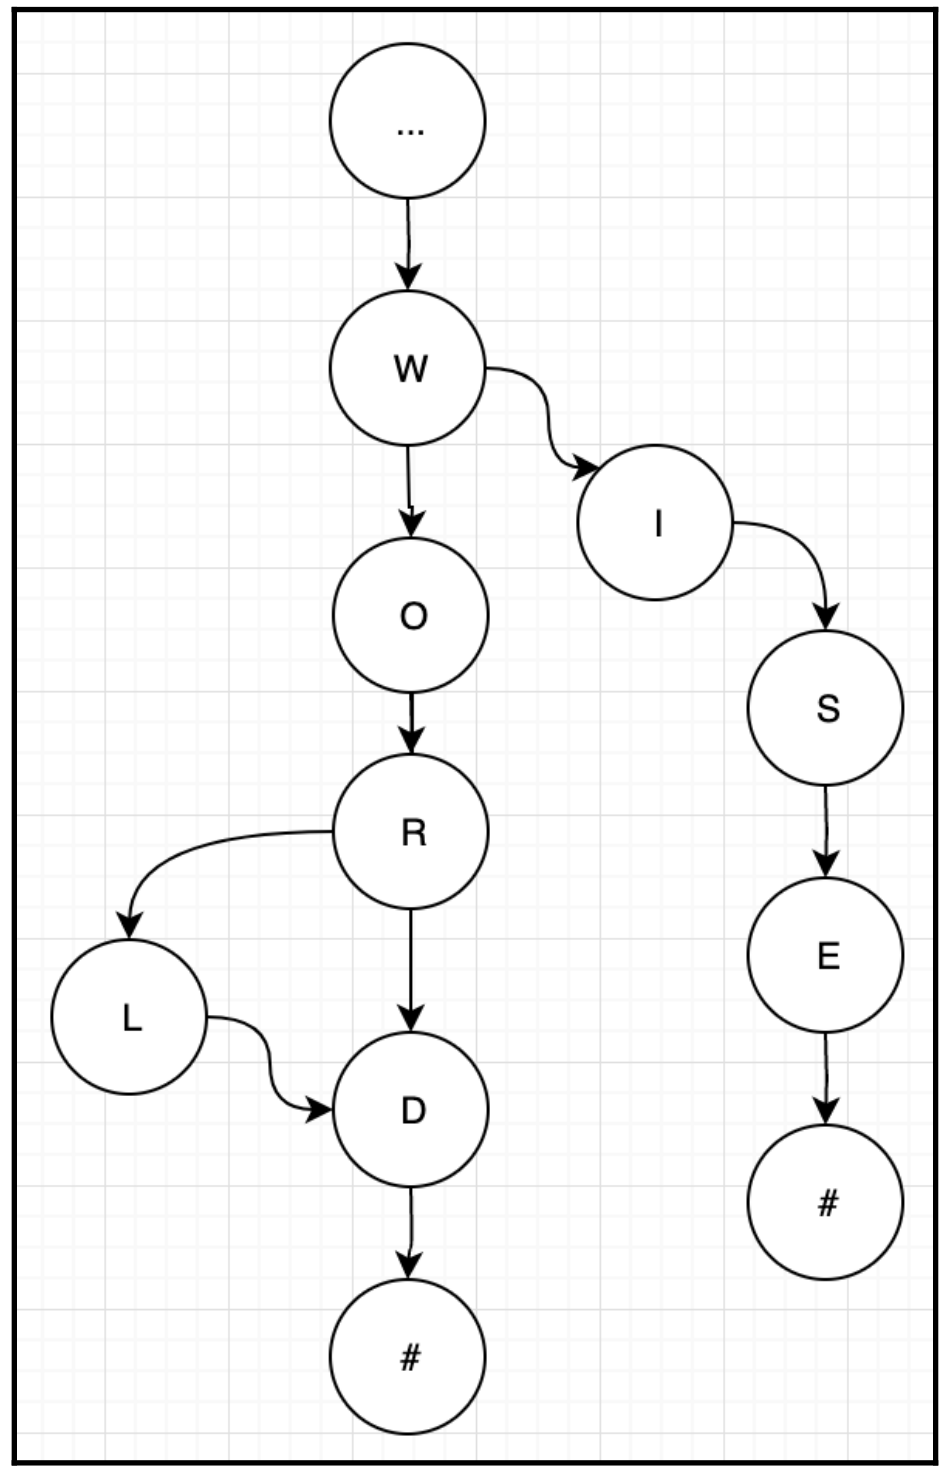
\includegraphics[width=0.6\textwidth]{content/Section-3/Chapter-16/6}
\end{center}

当引擎遇到world时,它将经历之前的尝试。w很好,o也很好,直到单词l中的倒数第二个字符为止,其他的一切都很好。在前面的图中,l之后没有终端节点,只有d。这意味着我们确定不存在world这样的单词,所以它可能是world。为了提供好的建议和检查拼写错误,我们应该有一个完整的用户语言词汇词典。当您计划支持多种语言时,这将变得更加困难。然而,虽然收集和存储字典是一项容易的任务,但更难的任务是收集Web上的所有文档并相应地存储它们以执行快速搜索。收集和解析网站以构建搜索引擎数据库(如前所述)的搜索引擎的工具、程序或模块称为爬虫程序。在深入了解存储这些网站页面的方式之前,让我们先快速了解一下爬虫程序的功能。 \par

\noindent\textbf{}\ \par
\textbf{爬虫} \ \par
每次用户输入查询时搜索数百万个文档是不现实的。想象一个搜索引擎,在用户点击系统UI上的搜索按钮之后,它解析网站以搜索用户查询。那将永远无法完成。搜索引擎对网站的每个请求都需要一些时间。即使它小于1毫秒(0.001秒),在用户等待查询完成时,分析和解析所有网站也需要很长的时间。为了让事情更清楚,让我们假设访问和搜索一个网站大约需要0.5毫秒(即使这样,那也是不合理的快)。这意味着搜索100万个网站大约需要8分钟。现在想象一下你打开一个谷歌搜索并进行查询——你会等待8分钟吗? \par
正确的方法是将所有信息存储在数据库中,以便搜索引擎有效地访问。爬虫程序下载网站页面并将其存储为临时文档,直到进行解析和建立索引。复杂的爬虫程序还会对文档进行解析,以使它们保持对索引器更方便的格式。这里重要的一点是,下载一个网页不是一个只发生一次的操作。Web页面的内容可能会更新。同时,在此期间可能会出现新的页面。因此,搜索引擎必须保持其数据库的更新。为了实现这一点,它安排爬虫程序定期下载页面。聪明的爬虫程序可能会在将内容传递给索引器之前比较内容的不同之处。 \par
通常,爬虫程序作为多线程应用程序工作。开发人员应该注意使爬行尽可能快,因为保持数十亿文档的最新不是一项容易的任务。正如我们已经提到的,搜索引擎并不直接搜索文档。它在所谓的索引文件中执行搜索。虽然爬行是一项有趣的编码任务,但在本章中,我们将关注于索引。下一节将介绍搜索引擎中的索引。 \par

\noindent\textbf{}\ \par
\textbf{索引文件} \ \par
搜索引擎的关键功能是索引。下面的图表显示了爬虫程序如何处理下载的文档来构建索引文件: \par

\begin{center}
	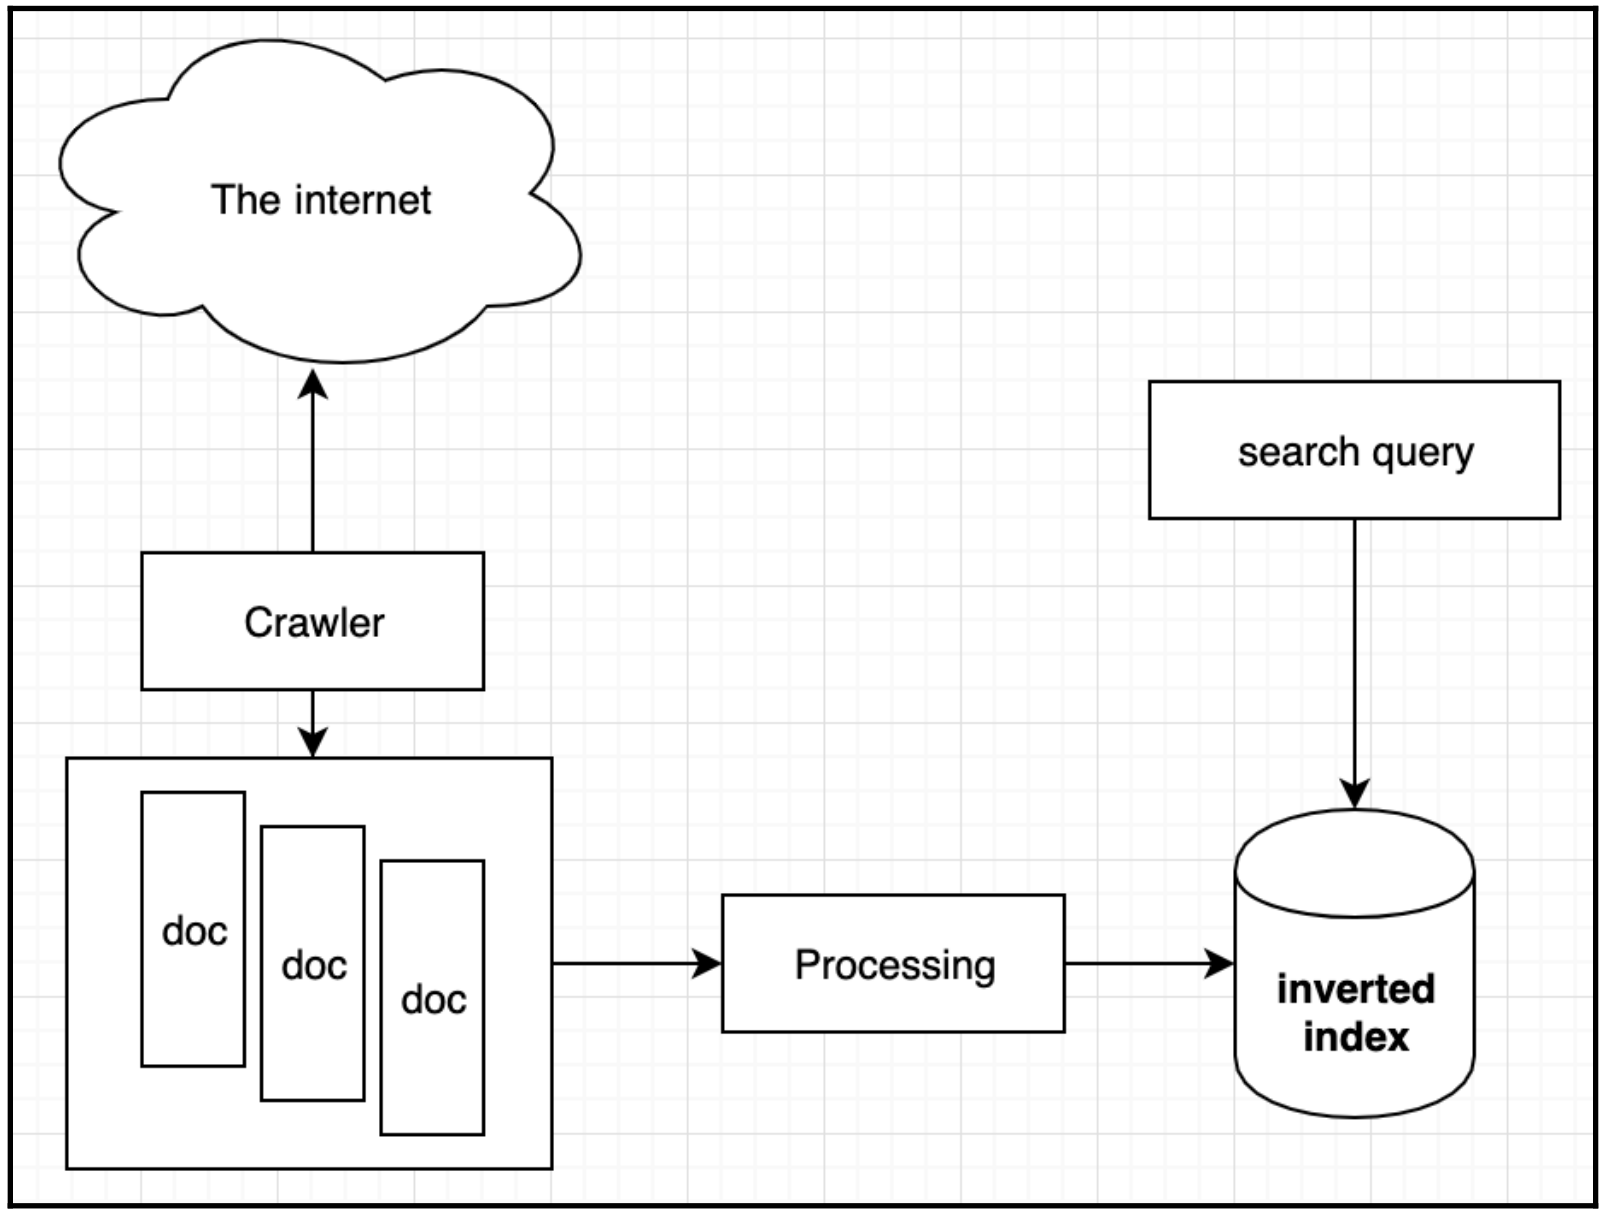
\includegraphics[width=0.8\textwidth]{content/Section-3/Chapter-16/7}
\end{center}

上面的图表中,索引显示为反向索引,用户查询被定向到反向索引。虽然我们在本章中交替使用索引和倒序索引,但反向索引是一个更准确的名称。首先,让我们看看搜索引擎的索引是什么。建立文档索引的全部原因是为了提供快速搜索功能。其思想很简单:每次爬虫程序下载文档时,搜索引擎都会处理它的内容,将其划分为引用该文档的单词。这个过程称为标记化。假设我们从维基百科下载了一个包含以下文本的文档(为了简洁起见,我们只取一部分作为例子): \par

\begin{lstlisting}[caption={}]
In 1979, Bjarne Stroustrup, a Danish computer scientist, began work on "C with Classes", the predecessor to C++. The motivation for creating a new language originated from Stroustrup's experience in programming for his PhD thesis. Stroustrup found that Simula had features that were very helpful for large software development...
\end{lstlisting}

搜索引擎将前面的文档分成几个单独的单词,如下所示(为了简洁起见,这里只显示前几个单词): \par

\begin{lstlisting}[caption={}]
In
1979
Bjarne
Stroustrup
a
Danish
computer
scientist
began
work
...
\end{lstlisting}

在将文档划分为单词之后,引擎将为文档中的每个单词分配一个标识符(ID)。假设前面文档的ID为1,下表显示了单词引用(出现在)ID为1的文档中: \par

\begin{table}[h]
	\begin{tabularx}{\textwidth}{|X|X|}
	\hline
	In & 1 \\
	\hline
	1979 & 1 \\
	\hline
	Bjarne & 1 \\
	\hline
	Stroustrup & 1 \\
	\hline
	a & 1 \\
	\hline
	Danish & 1 \\
	\hline
	computer & 1 \\
	\hline
	scientist & 1 \\
	\hline
	... &  \\
	\hline
	\end{tabularx}
\end{table}

可能有几个文档包含相同的单词,所以上面的表可能看起来更像下面的表: \par

\begin{table}[h]
	\begin{tabularx}{\textwidth}{|X|X|}
		\hline
		In & 1,4,14,22 \\
		\hline
		1979 & 1,99,455 \\
		\hline
		Bjarne & 1,202,1314 \\
		\hline
		Stroustrup & 1,1314 \\
		\hline
		a & 1,2,3,4,5,6,7,8,9,10,11,... \\
		\hline
		Danish & 1,99,102,103 \\
		\hline
		computer & 1,4,5,6,24,38,... \\
		\hline
		scientist & 1,38, 101, 3958, ... \\
		\hline
	\end{tabularx}
\end{table}

下面的表表示反向索引。它将单词与爬虫程序下载的文档的id映射在一起。现在查找包含用户作为查询输入的单词的文档变得更快了。现在,当用户通过键入computer来查询引擎时,结果将基于从索引中检索到的ID生成,即$ 1,4,5,6,24,38,… $在上面的例子中。索引还有助于为更复杂的查询找到结果。例如,“计算机科学家”匹配以下文件: \par

\begin{table}[h]
	\begin{tabularx}{\textwidth}{|X|X|}
		\hline
		computer & \textbf{1},4,5,6,24,\textbf{38},... \\
		\hline
		scientist & \textbf{1},\textbf{38}, 101, 3958, ... \\
		\hline
	\end{tabularx}
\end{table}

要用包含两个术语的文档响应用户,我们应该找到引用文档的交集(参见上表中的粗体数字),例如1和38。 \par
注意,用户查询在与索引匹配之前也需要标记化。标记化通常涉及到词的规范化。如果没有规范化,计算机科学家查询将不会给出任何结果(注意查询中的大写字母)。让我们进一步了解一下。 \par

\noindent\textbf{}\ \par
\textbf{分词文件} \ \par
您可能还记得第1章中标记化的概念,其中我们讨论了编译器如何通过将源文件标记为更小的、不可分割的单元(称为标记)来解析源文件。搜索引擎以类似的方式解析和标记文档。 \par
我们不会过多地讨论这个问题,但是应该考虑到,文档的处理方式意味着标记(在搜索引擎上下文中具有意义的不可分割的术语)是规范化的。例如,我们正在查看的所有单词都是小写的。因此,索引表应该如下所示: \par

\begin{table}[h]
	\begin{tabularx}{\textwidth}{|X|X|}
		\hline
		in & 1,4,14,22 \\
		\hline
		1979 & 1,99,455 \\
		\hline
		bjarne & 1,202,1314 \\
		\hline
		stroustrup & 1,1314 \\
		\hline
		a & 1,2,3,4,5,6,7,8,9,10,11,... \\
		\hline
		danish & 1,99,102,103 \\
		\hline
		computer & 1,4,5,6,24,38,... \\
		\hline
		scientist & 1,38, 101, 3958, ... \\
		\hline
	\end{tabularx}
\end{table}

作为C++程序员,看到小写的bjarne或stroustrup可能会感到不舒服。然而,当我们用倒排的索引键匹配用户输入时,我们应该考虑到用户输入可能没有我们期望的形式。因此,我们需要对用户输入应用相同的规则,使其与倒排索引匹配。 \par
接下来,注意a,毫不夸张地说,这是每个文档中都会出现的一个词。其他的例子还有the, an, in等,我们把它们称为停止词。通常,搜索引擎会忽略它们,所以倒排索引会更新为以下形式: \par

\begin{table}[h]
	\begin{tabularx}{\textwidth}{|X|X|}
		\hline
		1979 & 1,99,455 \\
		\hline
		bjarne & 1,202,1314 \\
		\hline
		stroustrup & 1,1314 \\
		\hline
		danish & 1,99,102,103 \\
		\hline
		computer & 1,4,5,6,24,38,... \\
		\hline
		scientist & 1,38, 101, 3958, ... \\
		\hline
	\end{tabularx}
\end{table}

您应该注意,规范化不仅仅是使单词小写。它还包括将单词变为正常形式。 \par

\hspace*{\fill} \\ %插入空行

\includegraphics[width=0.05\textwidth]{images/warn}
将单词规范化为词根形式(或词干)也称为词干提取。 \par
\noindent\textbf{}\ \par

看看我们在本节开始时所使用的文件中的以下句子: \par

\begin{lstlisting}[caption={}]
The motivation for creating a new language originated from Stroustrup's experience in programming for his PhD thesis.
\end{lstlisting}

creation、originated和Stroustrup都是规范化的,所以反向索引的形式如下: \par

\begin{table}[h]
	\begin{tabularx}{\textwidth}{|X|X|}
		\hline
		motivation & 1 \\
		\hline
		create & 1 \\
		\hline
		new & 1 \\
		\hline
		language & 1 \\
		\hline
		originate & 1 \\
		\hline
		stroustrup & 1 \\
		\hline
		experience & 1 \\
		\hline
		programming & 1 \\
		\hline
		phd & 1 \\
		\hline
		thesis & 1 \\
		\hline
	\end{tabularx}
\end{table}

请注意,我们忽略了停止词,也没有在前面的表中包含。 \par
标记化是创建索引的第一步。除此之外,我们可以自由地以任何使搜索更好的方式处理输入。 \par

\noindent\textbf{}\ \par
\textbf{结果排序} \ \par
相关性是搜索引擎最重要的特性之一。仅响应与用户输入匹配的文档是不够的。我们应该对它们进行排序,使最相关的文档排在前面。 \par
一种策略是记录每个单词在文档中出现的次数。例如,描述计算机的文档可能包含单词computer的多次出现,如果用户搜索计算机,结果将首先显示包含最多的computer的文档。下面是一个索引表的例子: \par

\begin{table}[h]
	\begin{tabularx}{\textwidth}{|X|X|}
		\hline
		computer & 1\{18\}, 4\{13\}, 899\{3\} \\
		\hline
		map & 4\{9\}, 1342\{4\}, 1343\{2\} \\
		\hline
		world & 12\{1\} \\
		\hline
	\end{tabularx}
\end{table}

花括号中的值定义了文档中每个单词出现的次数。 \par
向用户展示搜索结果时,我们可以考虑许多因素。一些搜索引擎存储用户相关信息,以响应个性化的结果。甚至用户用于访问搜索引擎(通常是Web浏览器)的程序也可能改变搜索平台的结果,例如:在Linux操作系统上搜索重新安装操作系统的用户会得到列表顶部包含重新安装Ubuntu的结果,因为浏览器向搜索引擎提供了操作系统类型和版本信息。然而,考虑到隐私问题,有些搜索引擎完全不使用个性化用户数据。 \par
文档的另一个属性是更新日期,新鲜内容总是具有更高的优先级。因此,当向用户返回一个文档列表时,我们还可以按照其内容更新的顺序对它们重新排序。考虑到文档的相关排名,我们将进入下一节,在这里我们将讨论推荐引擎。 \par

\noindent\textbf{}\ \par
\textbf{构建推荐引擎} \ \par
在前一章中,我们介绍了人工智能(AI)和机器学习(ML)。推荐引擎可以视为人工智能驱动的解决方案或简单的条件语句集合。构建一个接受用户数据并返回最满足输入的选项的系统是一项复杂的任务。将ML合并到这样的任务中,可能很合理。 \par
但是,您应该考虑这样一个事实:推荐引擎可能包含一组规则,在将数据输出给最终用户之前,根据这些规则对数据进行处理。推荐引擎可以在预期和意外的地方运行。例如,在Amazon上浏览产品时,推荐引擎会根据我们当前浏览的产品向我们推荐产品。电影数据库会根据我们之前看过的电影或分级的电影来推荐新的电影。这对许多人来说可能是意想不到的,但推荐引擎也运行在搜索引擎之后。 \par
你可能熟悉一些电子商务平台推荐产品的方式。大多数时候,建议面板的标题是类似于购买了这个的客户,也购买了....回想一下我们在前一章介绍过的聚类分析。现在,如果我们试图理解这些建议是如何在幕后工作的,我们很可能会发现一些聚类算法。 \par
让我们简单地看一看,并尝试设计一些推荐机制。让我们以一个书店网站为例。John买了一本名为《精通Qt5》的书,所以让我们把这些信息放在下面的表格中: \par

\begin{table}[h]
	\begin{tabularx}{\textwidth}{|X|X|}
		\hline
		 & Mastering Qt5 \\
		\hline
		John & yes \\
		\hline
	\end{tabularx}
\end{table}

接下来,约翰决定买一本C++书《精通c++编程》。莱娅买了一本名为《设计模式》的书。卡尔买了三本书,分别是《学习Python》、《掌握机器学习》和《用Python学习机器》。表格会进行更新,现在看起来像这样: \par

\begin{table}[h]
	\begin{tabularx}{\textwidth}{|X|X|X|X|X|X|X|}
		\hline
		& Mastering Qt5 & Mastering	C++ Programming & Design	Patterns & Learning	Python & Mastering Machine Learning & Machine Learning with Python \\
		\hline
		John & yes & yes & no & no & no & no \\
		\hline
		Leia & no & no & yes & no & no & no \\
		\hline
		Karl & no & no & no & yes & yes & yes \\
		\hline
	\end{tabularx}
\end{table}

现在,让我们想象一下Harut访问了网站并购买了前面列出的两本书,《学习Python》和《用Python学习机器》。那么向他推荐《精通Qt5》这本书合理吗?我们不这么认为。但是我们知道他买了什么书,我们也知道另外一个用户Karl买了三本书,其中两本和Harut买的书是一样的。所以,向Harut推荐精通机器学习可能是合理的,告诉他买了其他两本书的顾客也买了这本书。这是一个简单的例子,说明了从高层次的角度推荐引擎是如何工作的。 \par

\noindent\textbf{}\ \par
\textbf{使用知识图谱} \ \par
现在,让我们回到搜索引擎。一个用户正在搜索一位著名的计算机科学家——比如Donald Knuth。他们在搜索字段中输入名称,然后从所有的Web中获得排序的结果,以提供最好的结果。我们再来看看谷歌搜索。为了充分利用用户界面,谷歌向我们展示了一些关于搜索主题的简要信息。在本例中,它在结果页面的右侧显示了这位伟大科学家的几张图片和一些关于他的信息。这部分看起来是这样的: \par

\begin{center}
	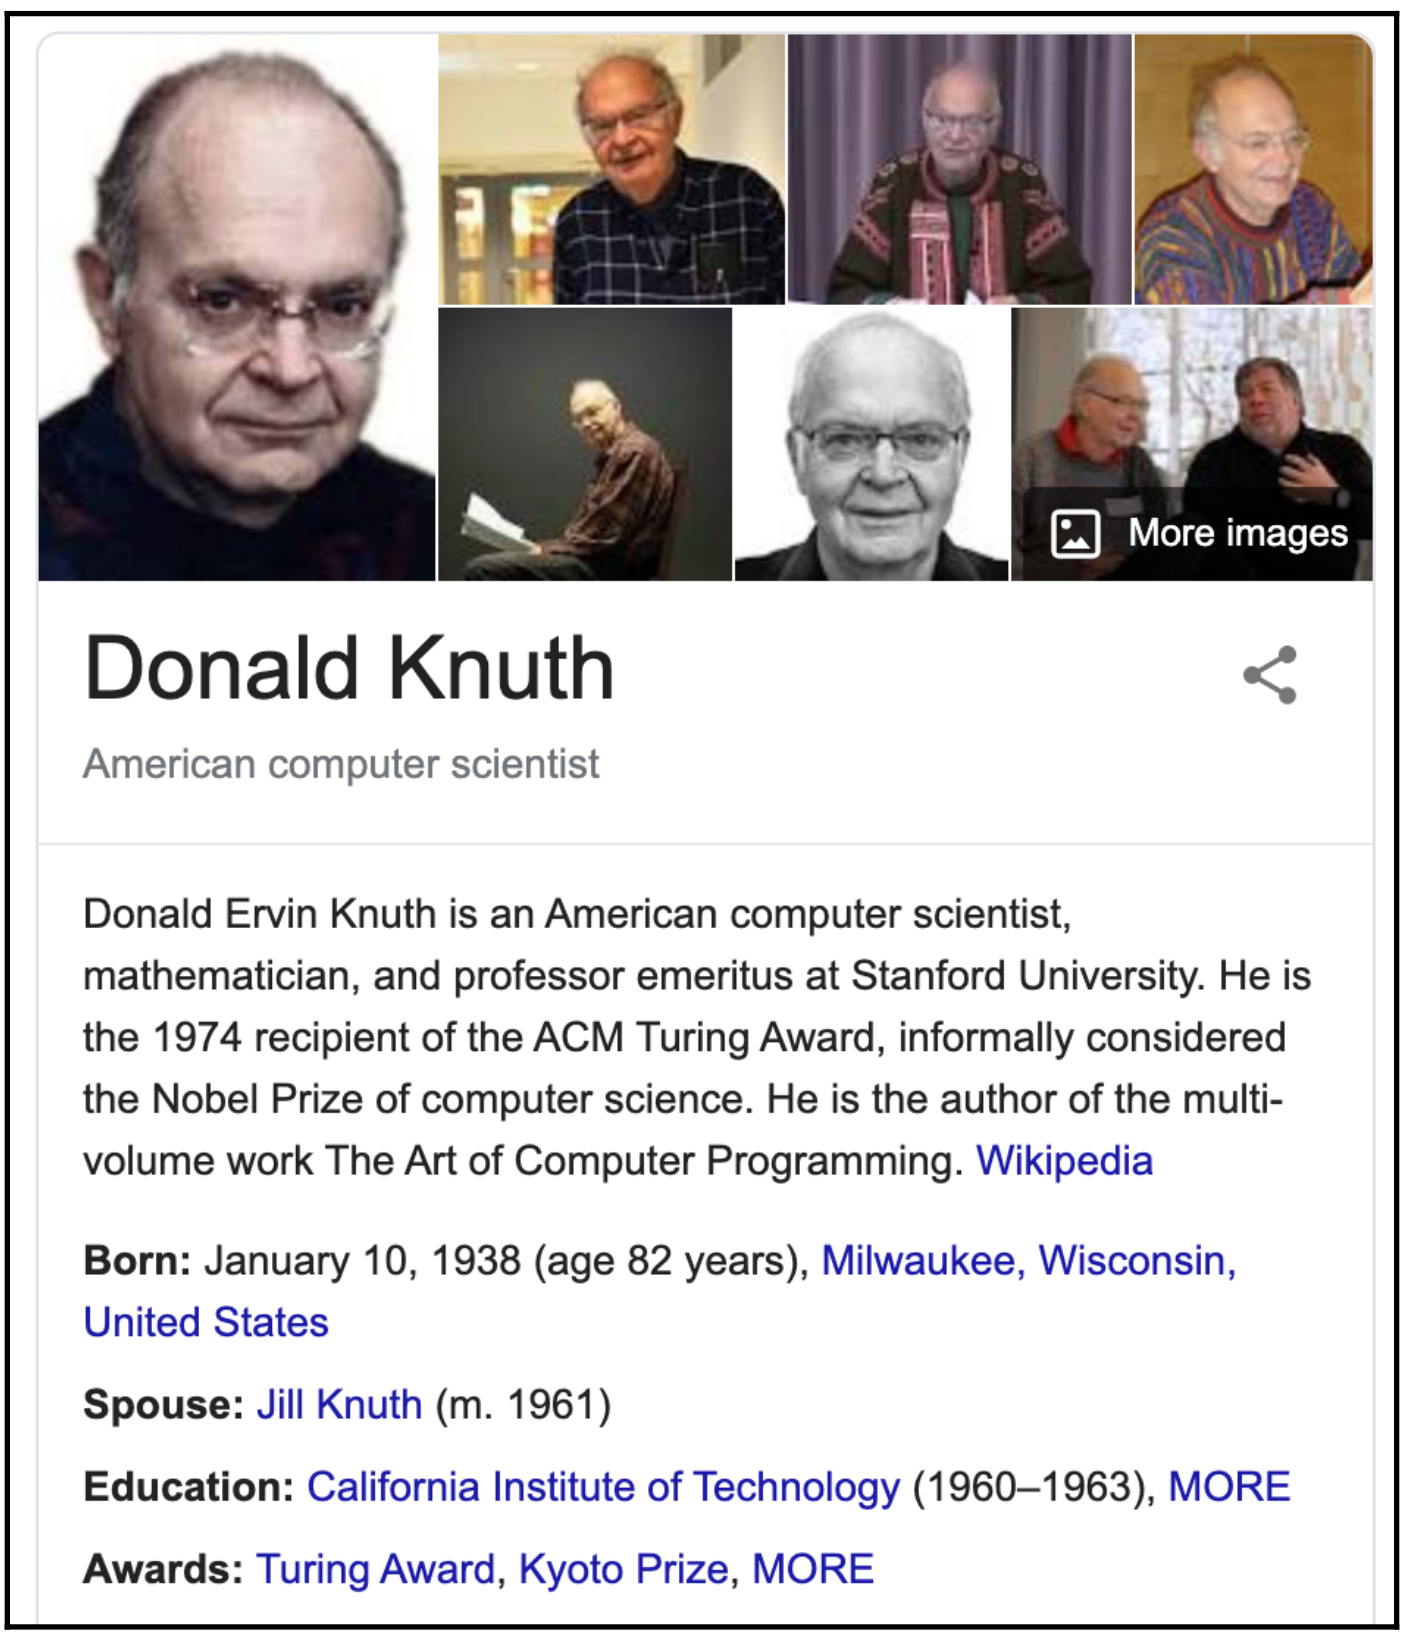
\includegraphics[width=0.8\textwidth]{content/Section-3/Chapter-16/8}
\end{center}

通过这种方式,搜索引擎试图满足用户的基本需求,让他们在不访问任何网站的情况下更快地找到信息。在这种情况下,我们最感兴趣的是放在前面信息框下面的建议框。它的标题是“人们也会搜索”,它是这样的: \par

\begin{center}
	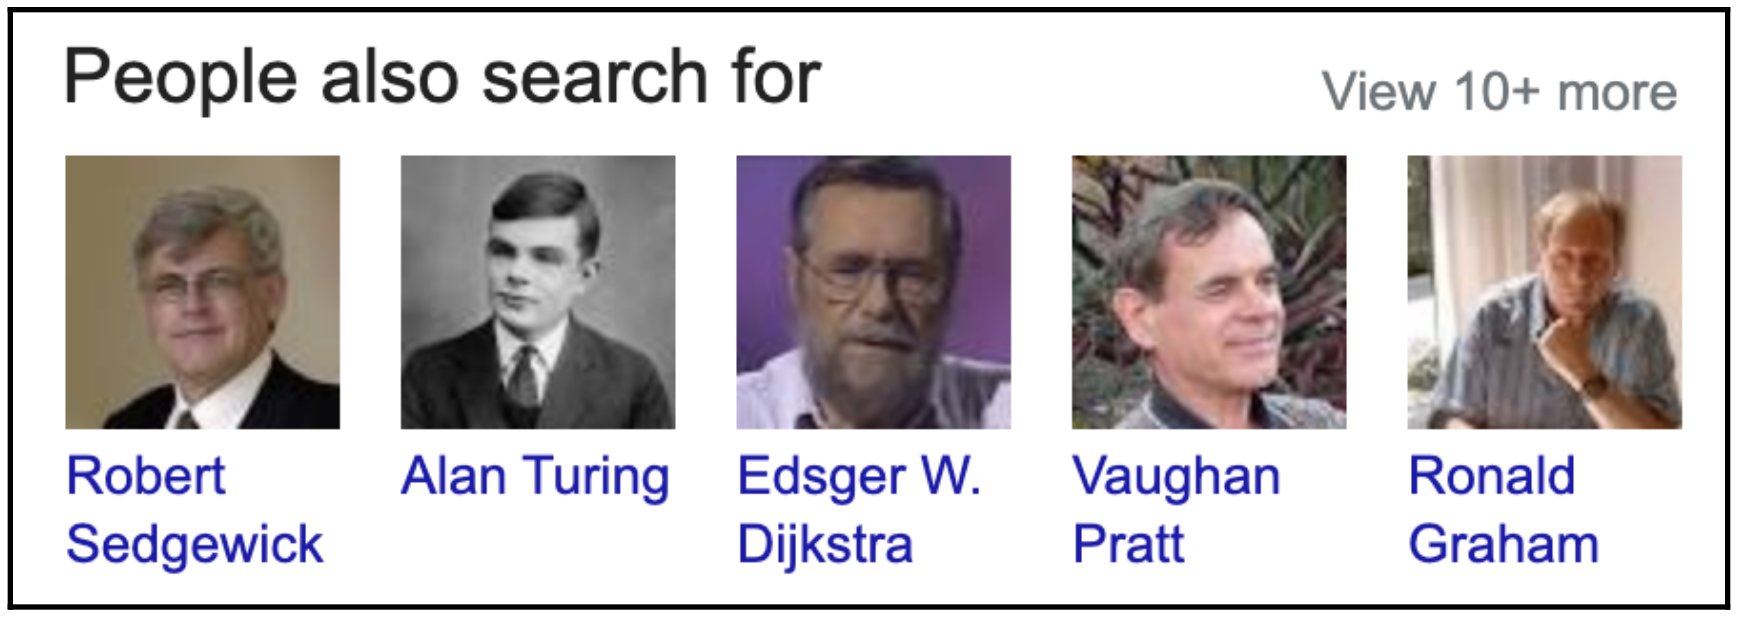
\includegraphics[width=0.8\textwidth]{content/Section-3/Chapter-16/9}
\end{center}

这些是基于用户搜索Alan·Turing的推荐,就在他们搜Donald·Knuth之后。这促使推荐引擎提出了一个建议,如果有人在搜索Donald·Knuth,他们可能也对Alan·Turing感兴趣。 \par
我们可以通过谷歌称之为知识图谱的东西来组织类似的建议机制。这是一个由节点组成的图,每个节点表示某个主题、人物、电影或其他可搜索的内容。图数据结构是节点和连接这些节点的边的集合,如下图所示: \par

\begin{center}
	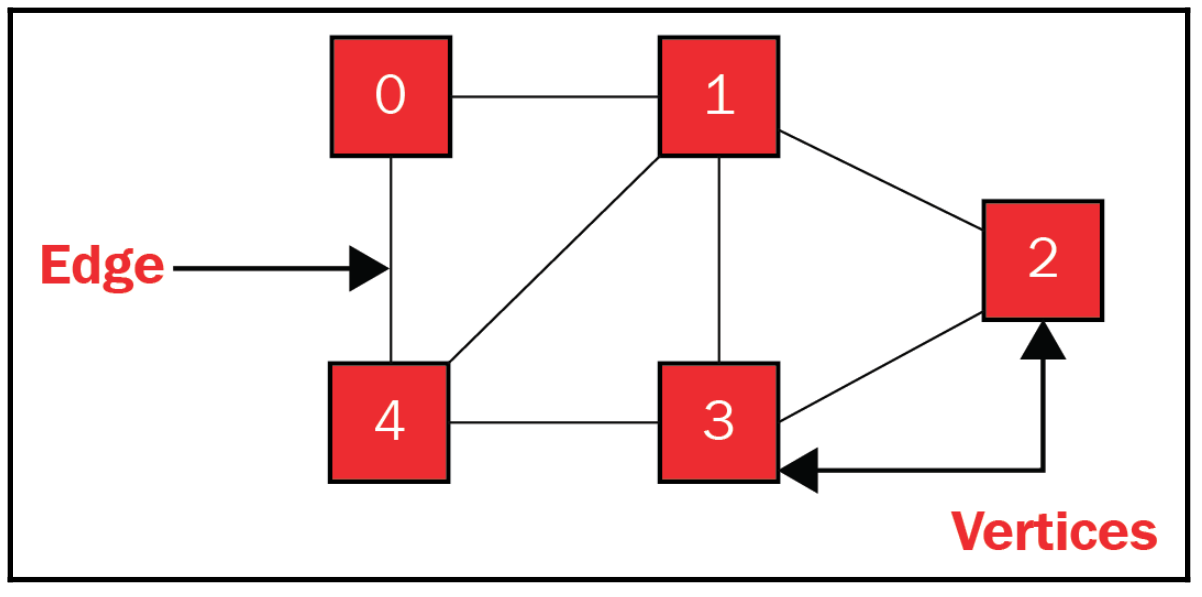
\includegraphics[width=0.8\textwidth]{content/Section-3/Chapter-16/10}
\end{center}

在知识图谱中,每个节点代表一个单独的实体。所谓实体,我们指的是一座城市,一个人,一只宠物,一本书,或者几乎任何你能想象到的东西。现在,图中的边表示实体之间的连接。每个节点可以通过多个节点连接到另一个节点。例如,看看这两个节点: \par

\begin{center}
	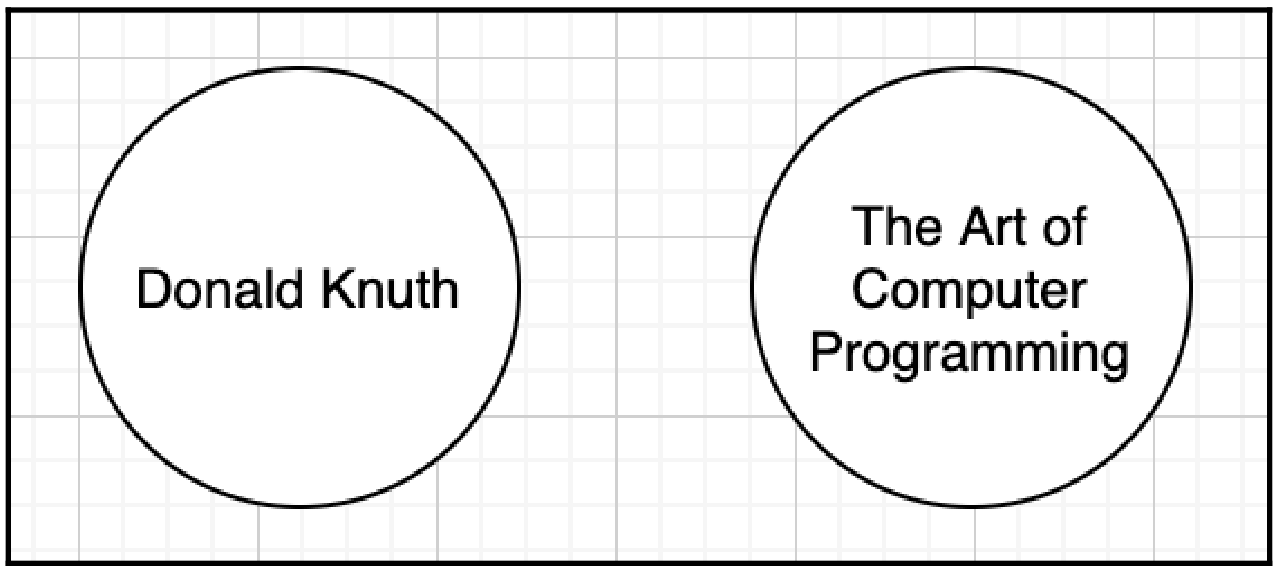
\includegraphics[width=0.8\textwidth]{content/Section-3/Chapter-16/11}
\end{center}

这两个节点只包含文本。我们可能会认为Donald·Knuth是一个名字,而《计算机编程的艺术》是某种艺术。构建知识图的本质是,我们可以将每个节点与表示其类型的另一个节点关联起来。下面的图是对前一图的扩展: \par

\begin{center}
	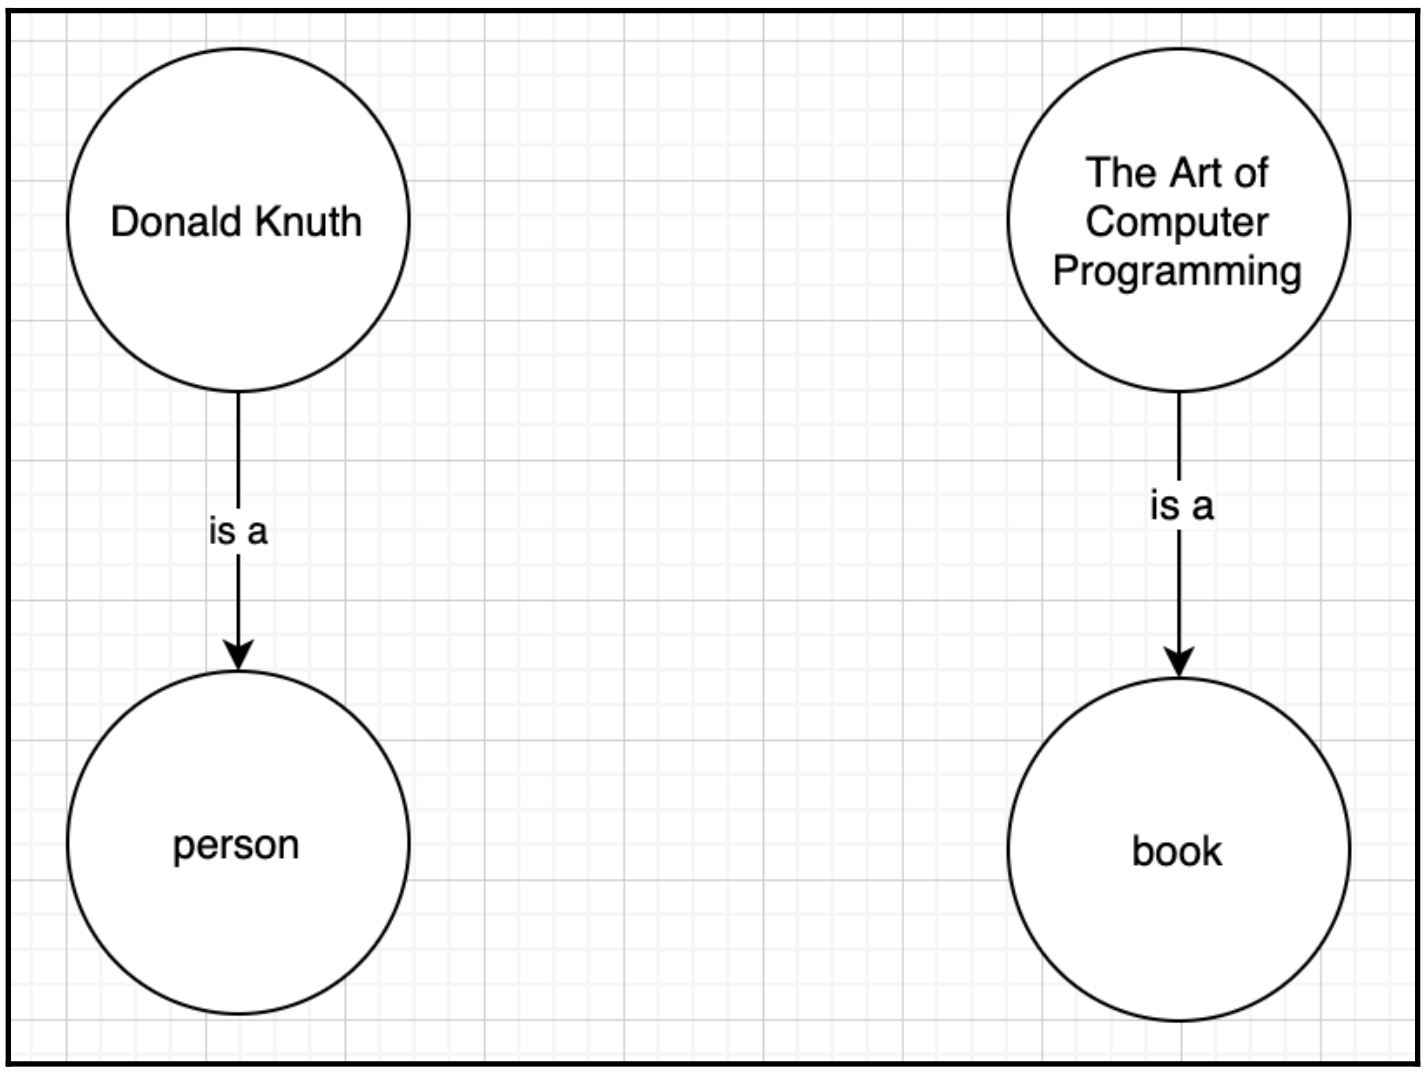
\includegraphics[width=0.8\textwidth]{content/Section-3/Chapter-16/12}
\end{center}

看看我们添加的两个新节点。其中一个代表一个人,而另一个代表一本书。更令人兴奋的是我们用一条边把Donald·Knuth节点和person节点连接起来并将其标记为'是'的关系。同样地,我们已经将《计算机编程艺术》节点与书籍节点连接起来,所以我们可以说计算机编程艺术是一本书。现在让我们把Donald·Knuth和他写的书联系起来: \par

\begin{center}
	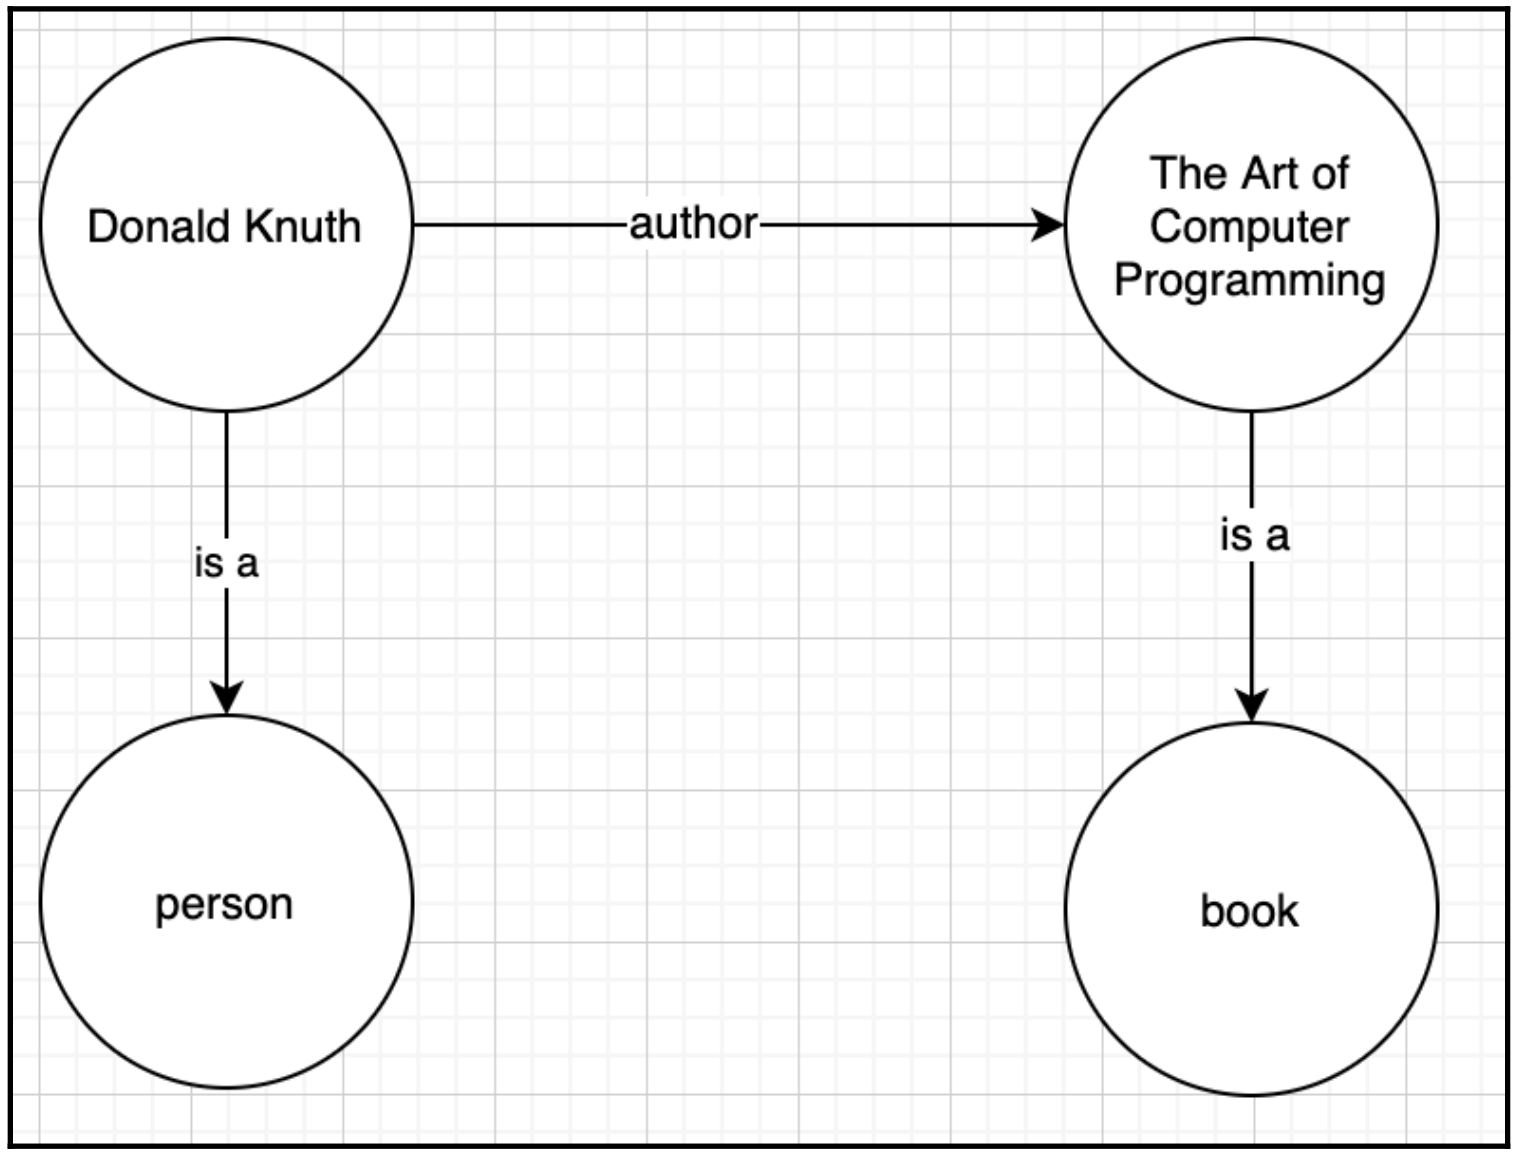
\includegraphics[width=0.8\textwidth]{content/Section-3/Chapter-16/13}
\end{center}

所以,现在我们有了一个完整的关系因为我们知道Donald·Knuth是《计算机编程艺术》的作者。\par
让我们再添加几个节点来表示人。下面的图表显示了我们是如何添加Alan·Turing和Peter·Weyland节点的: \par

\begin{center}
	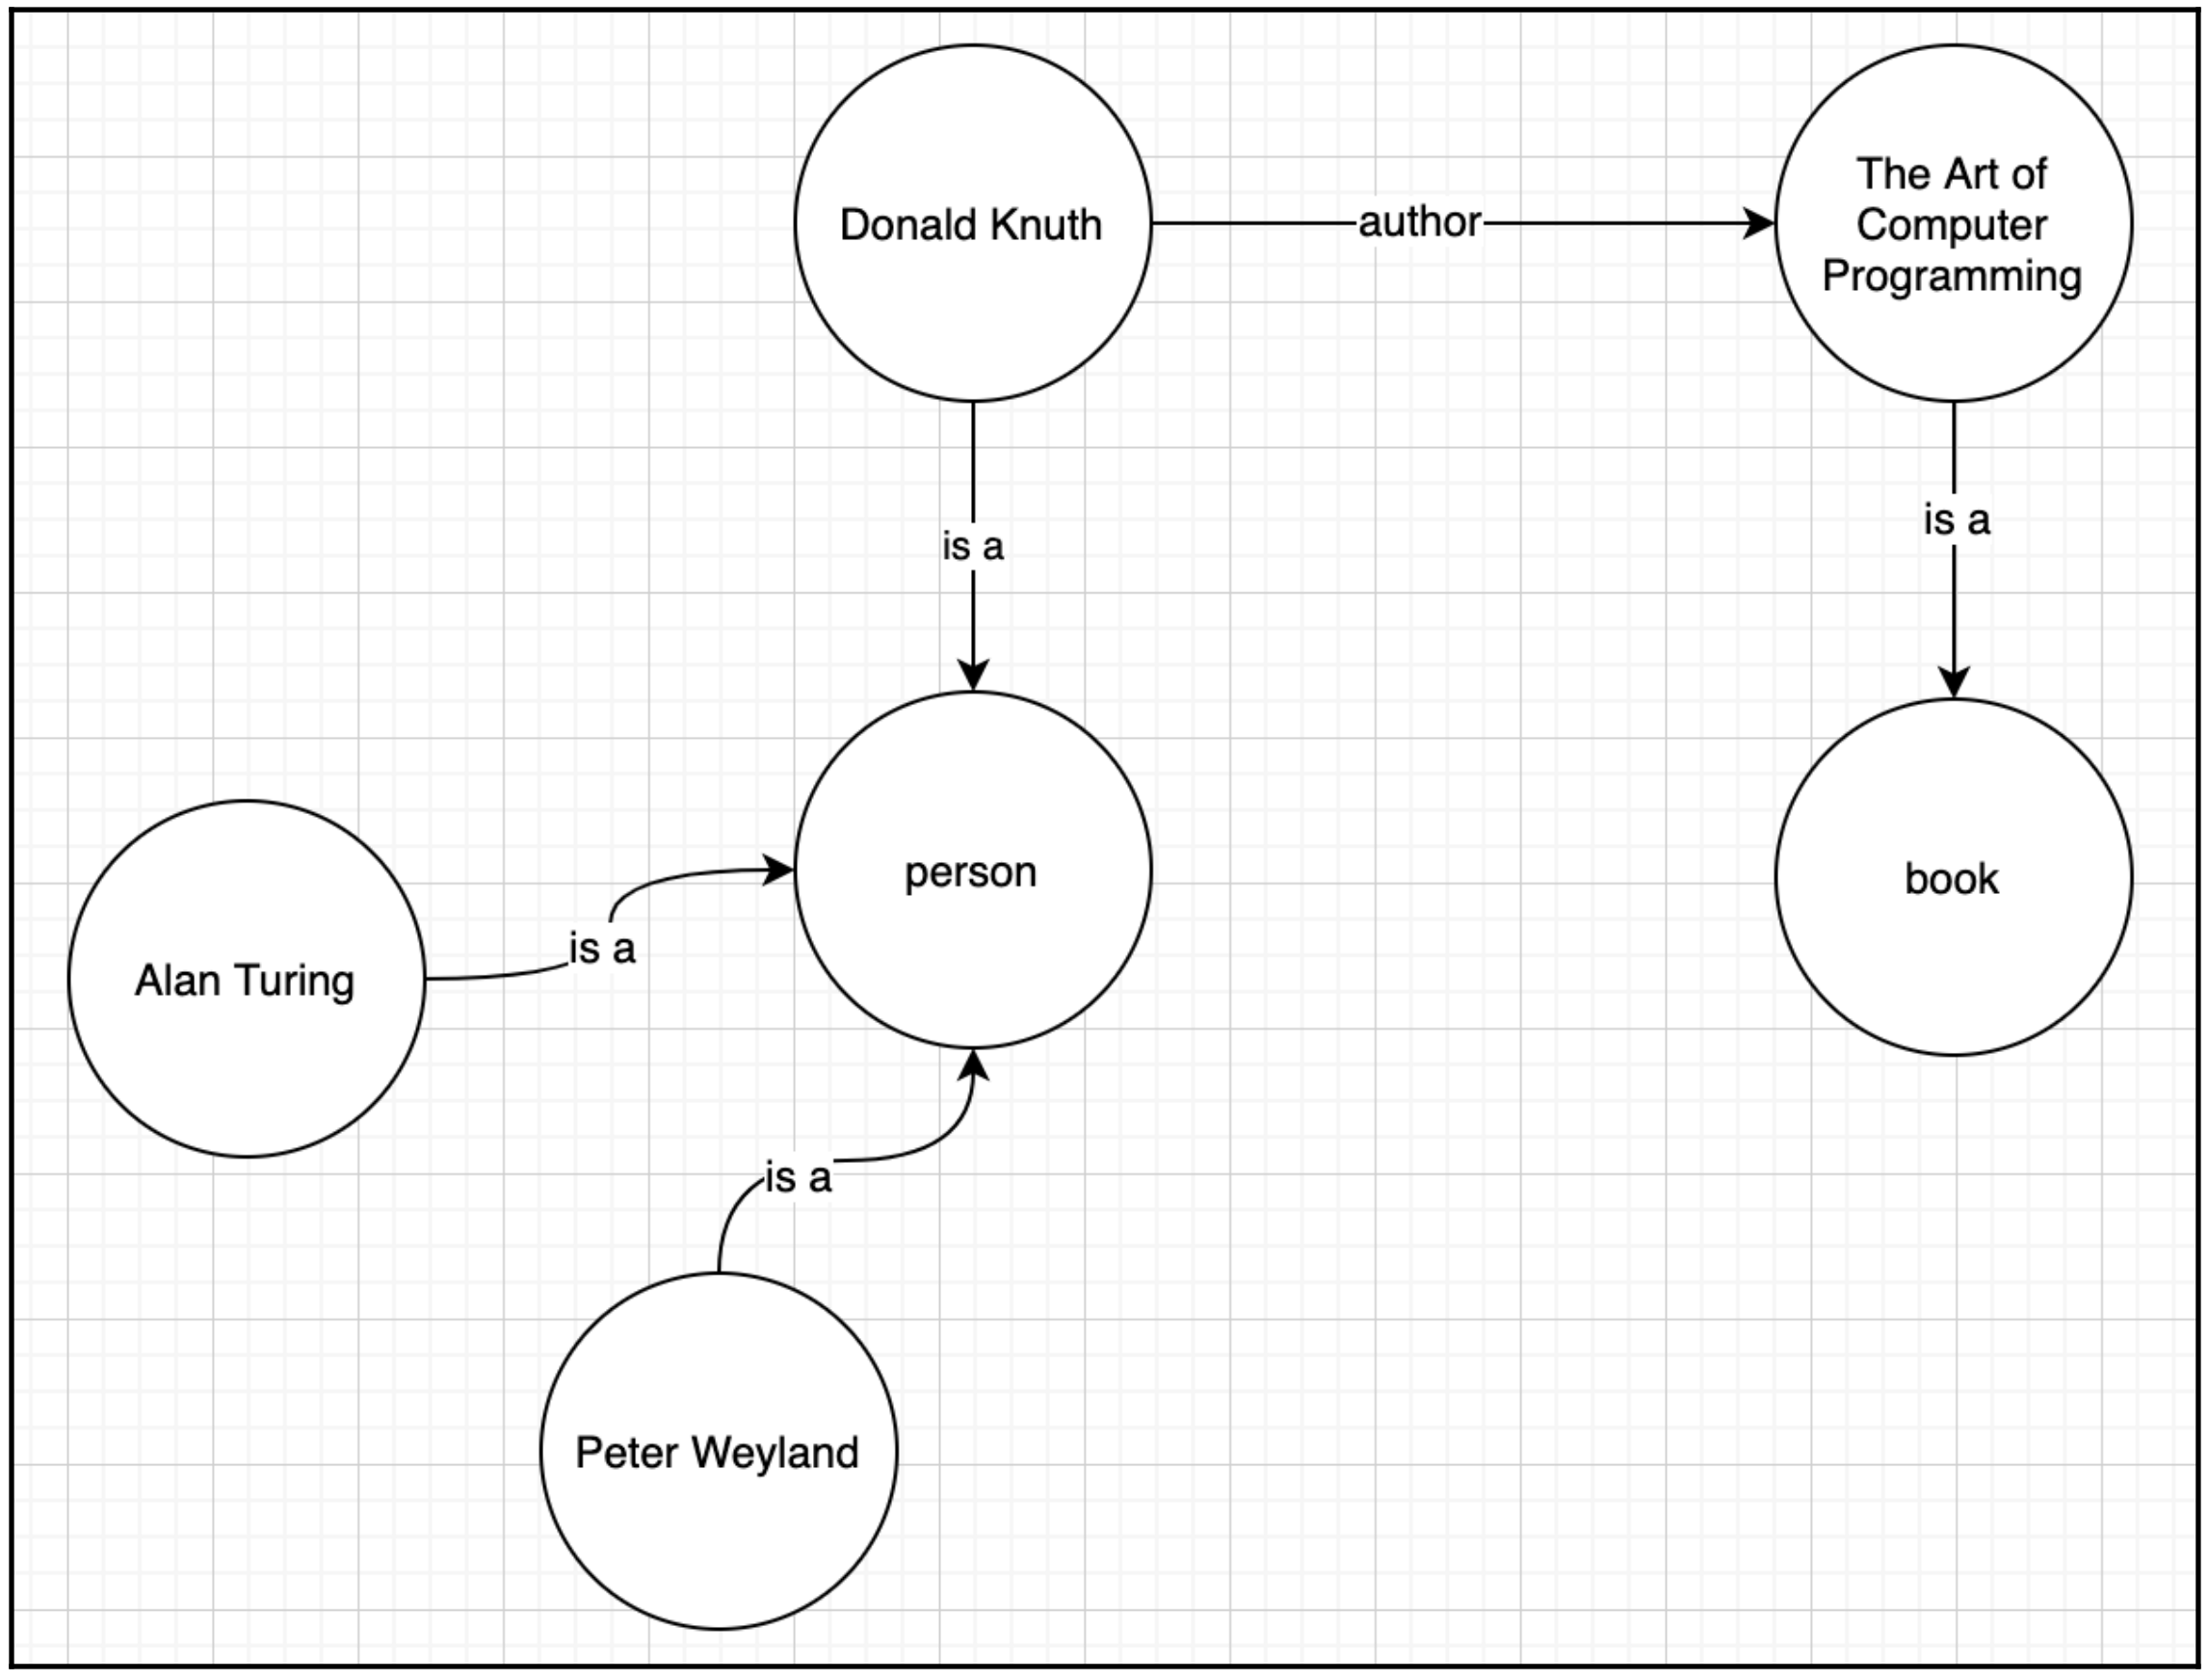
\includegraphics[width=0.8\textwidth]{content/Section-3/Chapter-16/14}
\end{center}

Alan·Turing和Peter·Weyland都是人。现在,如果这是搜索引擎知识库的一部分,那么它给了我们一个很好的洞察用户的搜索意图。当我们看到Donald·Knuth的结果时,我们知道这是关于一个人的。如果有必要,可以建议用户看看在知识图谱中已经积累的其他人。建议搜索Donald·Knuth的用户也看看Alan·Turing和Peter·Weyland的页面是否合理?好了,棘手的部分来了:尽管他们都是人,但他们之间的联系并不紧密。所以,我们需要一些额外的东西来定义两个不同的人之间的联系的相关性。看看图表中添加的以下内容: \par

\begin{center}
	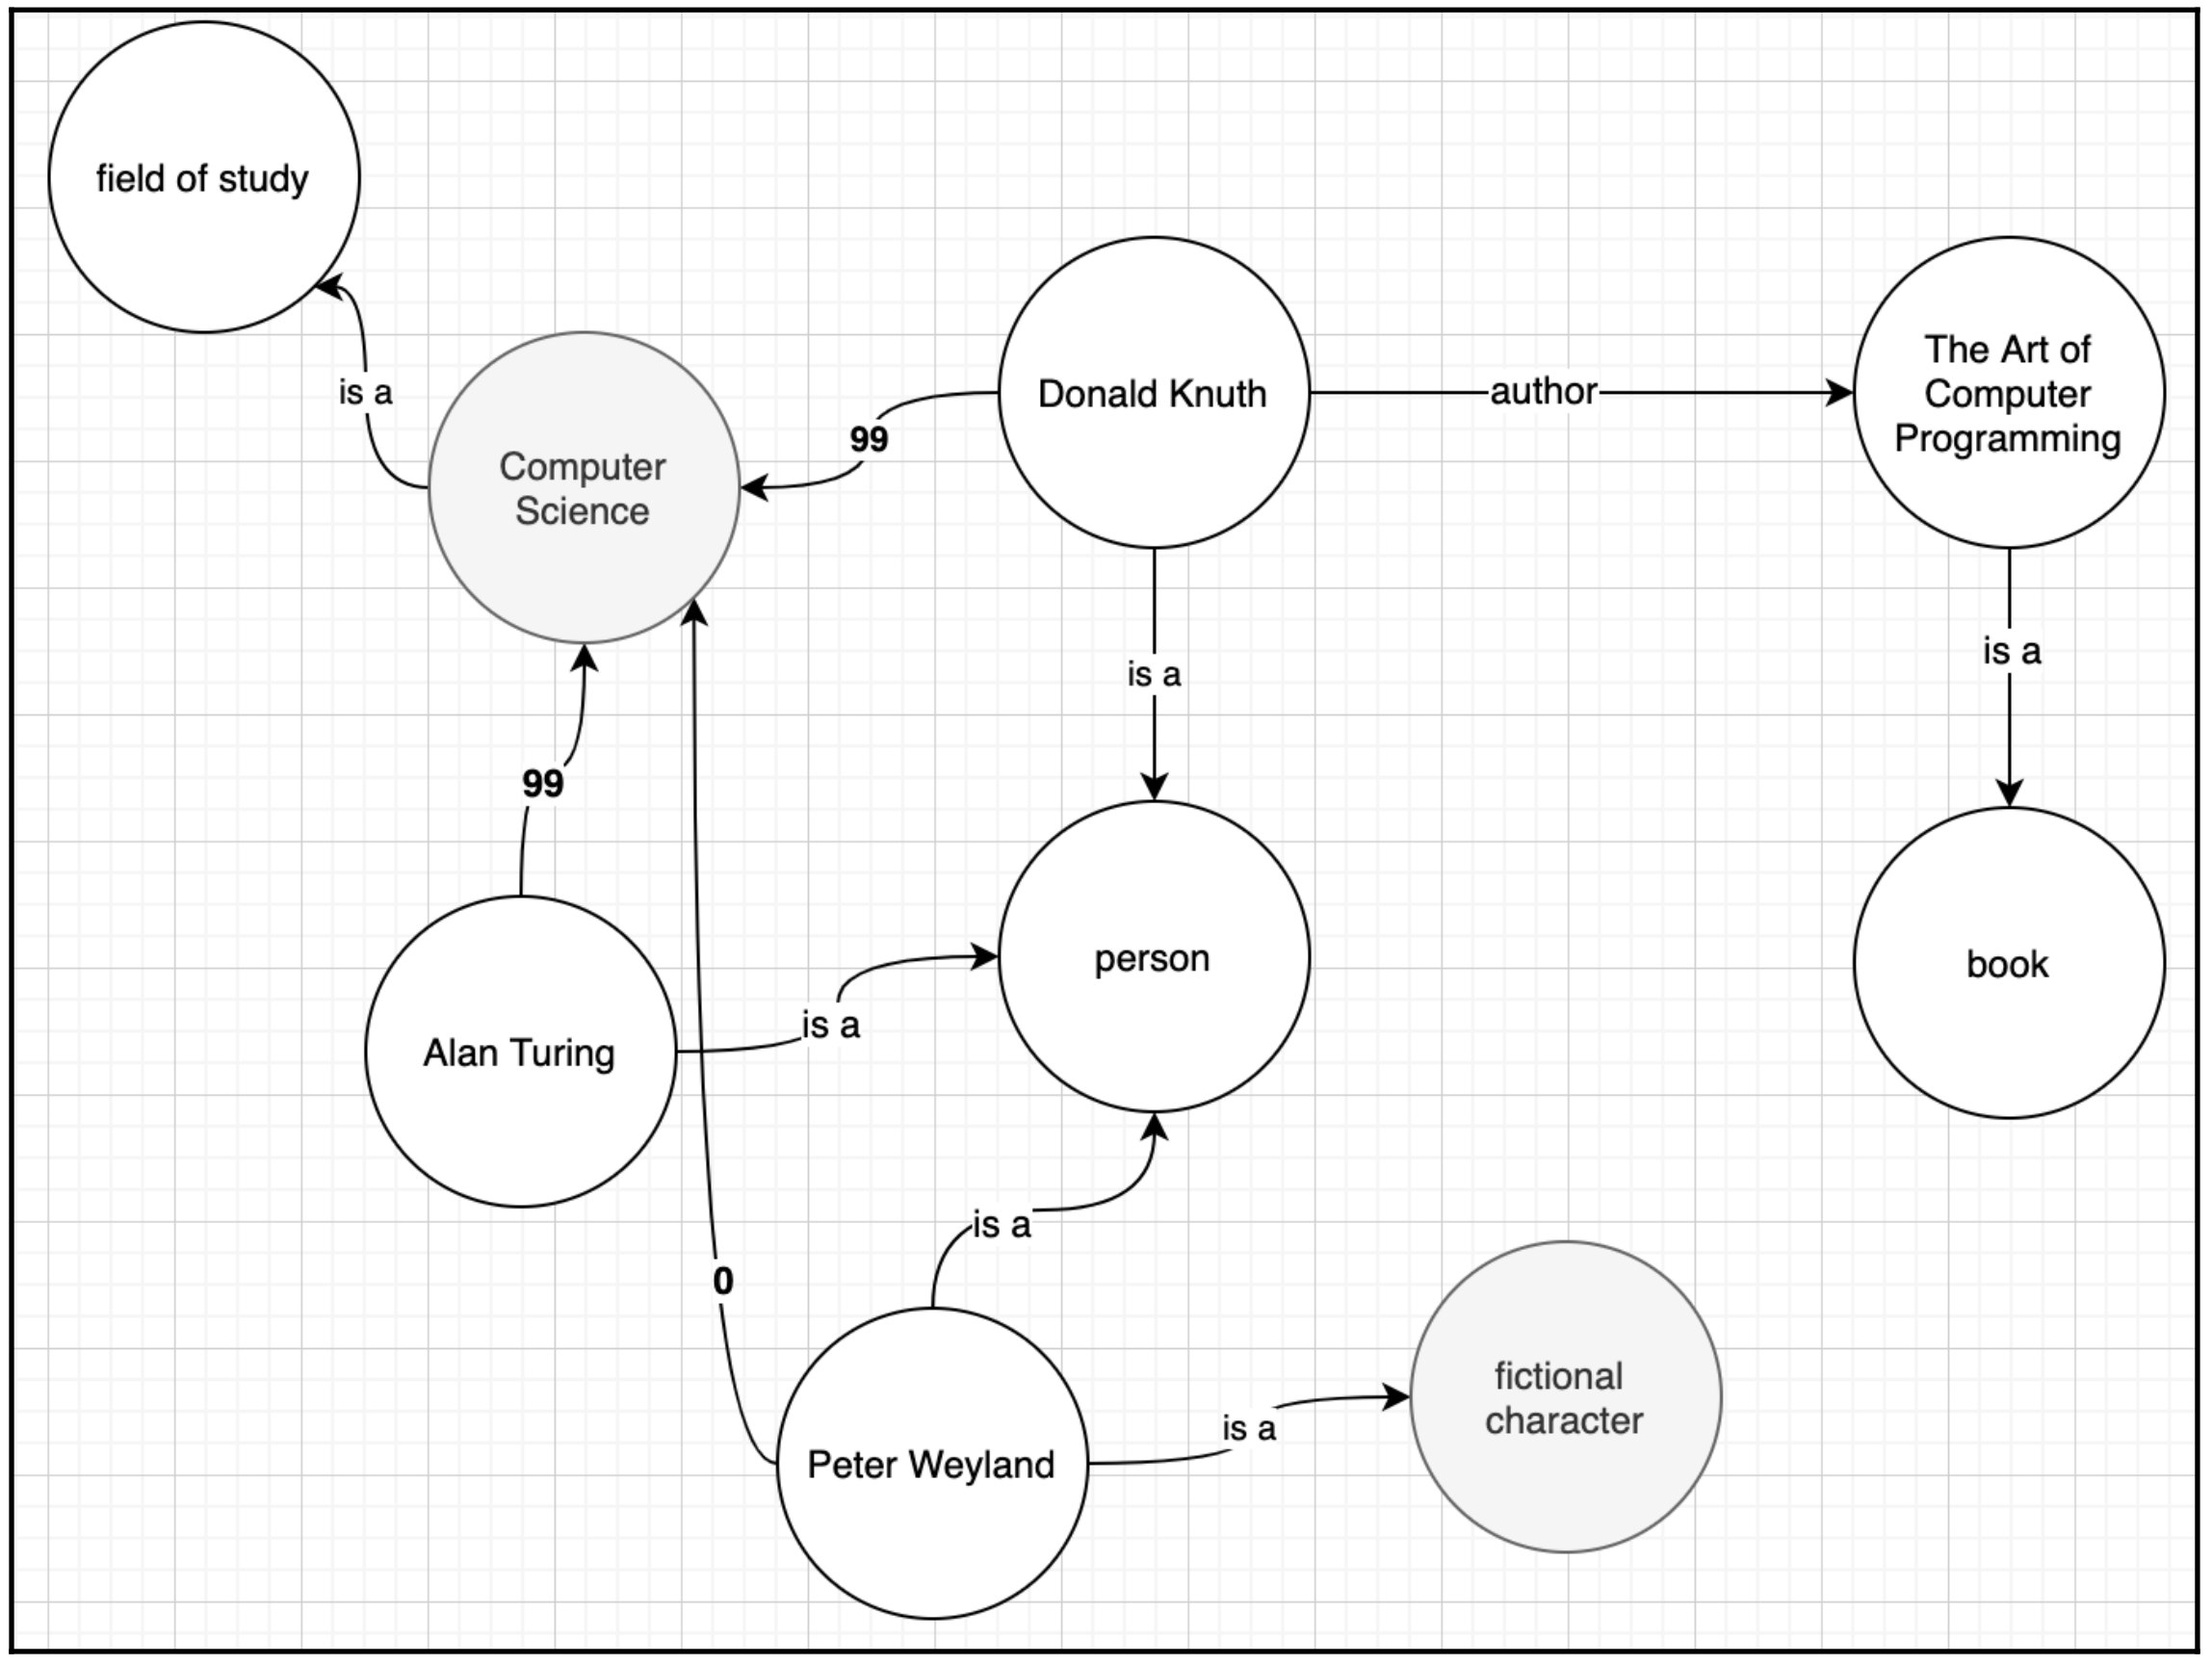
\includegraphics[width=0.8\textwidth]{content/Section-3/Chapter-16/15}
\end{center}

现在很清楚的是,Donald·Knuth和Alan·Turing的活动是相同的,作为计算机科学节点,代表了一个研究领域,而Peter·Weyland原来是一个虚构的人物。Peter·Weyland和Donald·Knuth唯一的联系就是他们都是人。看看我们放在从人节点到计算机科学节点的边缘上的数字。假设我们从0到100对这种关系进行评级,后者意味着这种关系是最强的。所以,我们给Alan·Turing和Donald·Knuth都加了99。我们应该忽略从Peter·Weyland到计算机科学的连线,而不是输入0,但我们这样做是为了显示对比。这些数字就是权重。我们在边缘添加权重以强调连接性因素,Donald·Knuth和Alan·Turing有相同的东西,而且彼此有很强的联系。如果我们把Steve·Jobs作为一个新人加入到知识图谱中,图谱会是这样的: \par

\begin{center}
	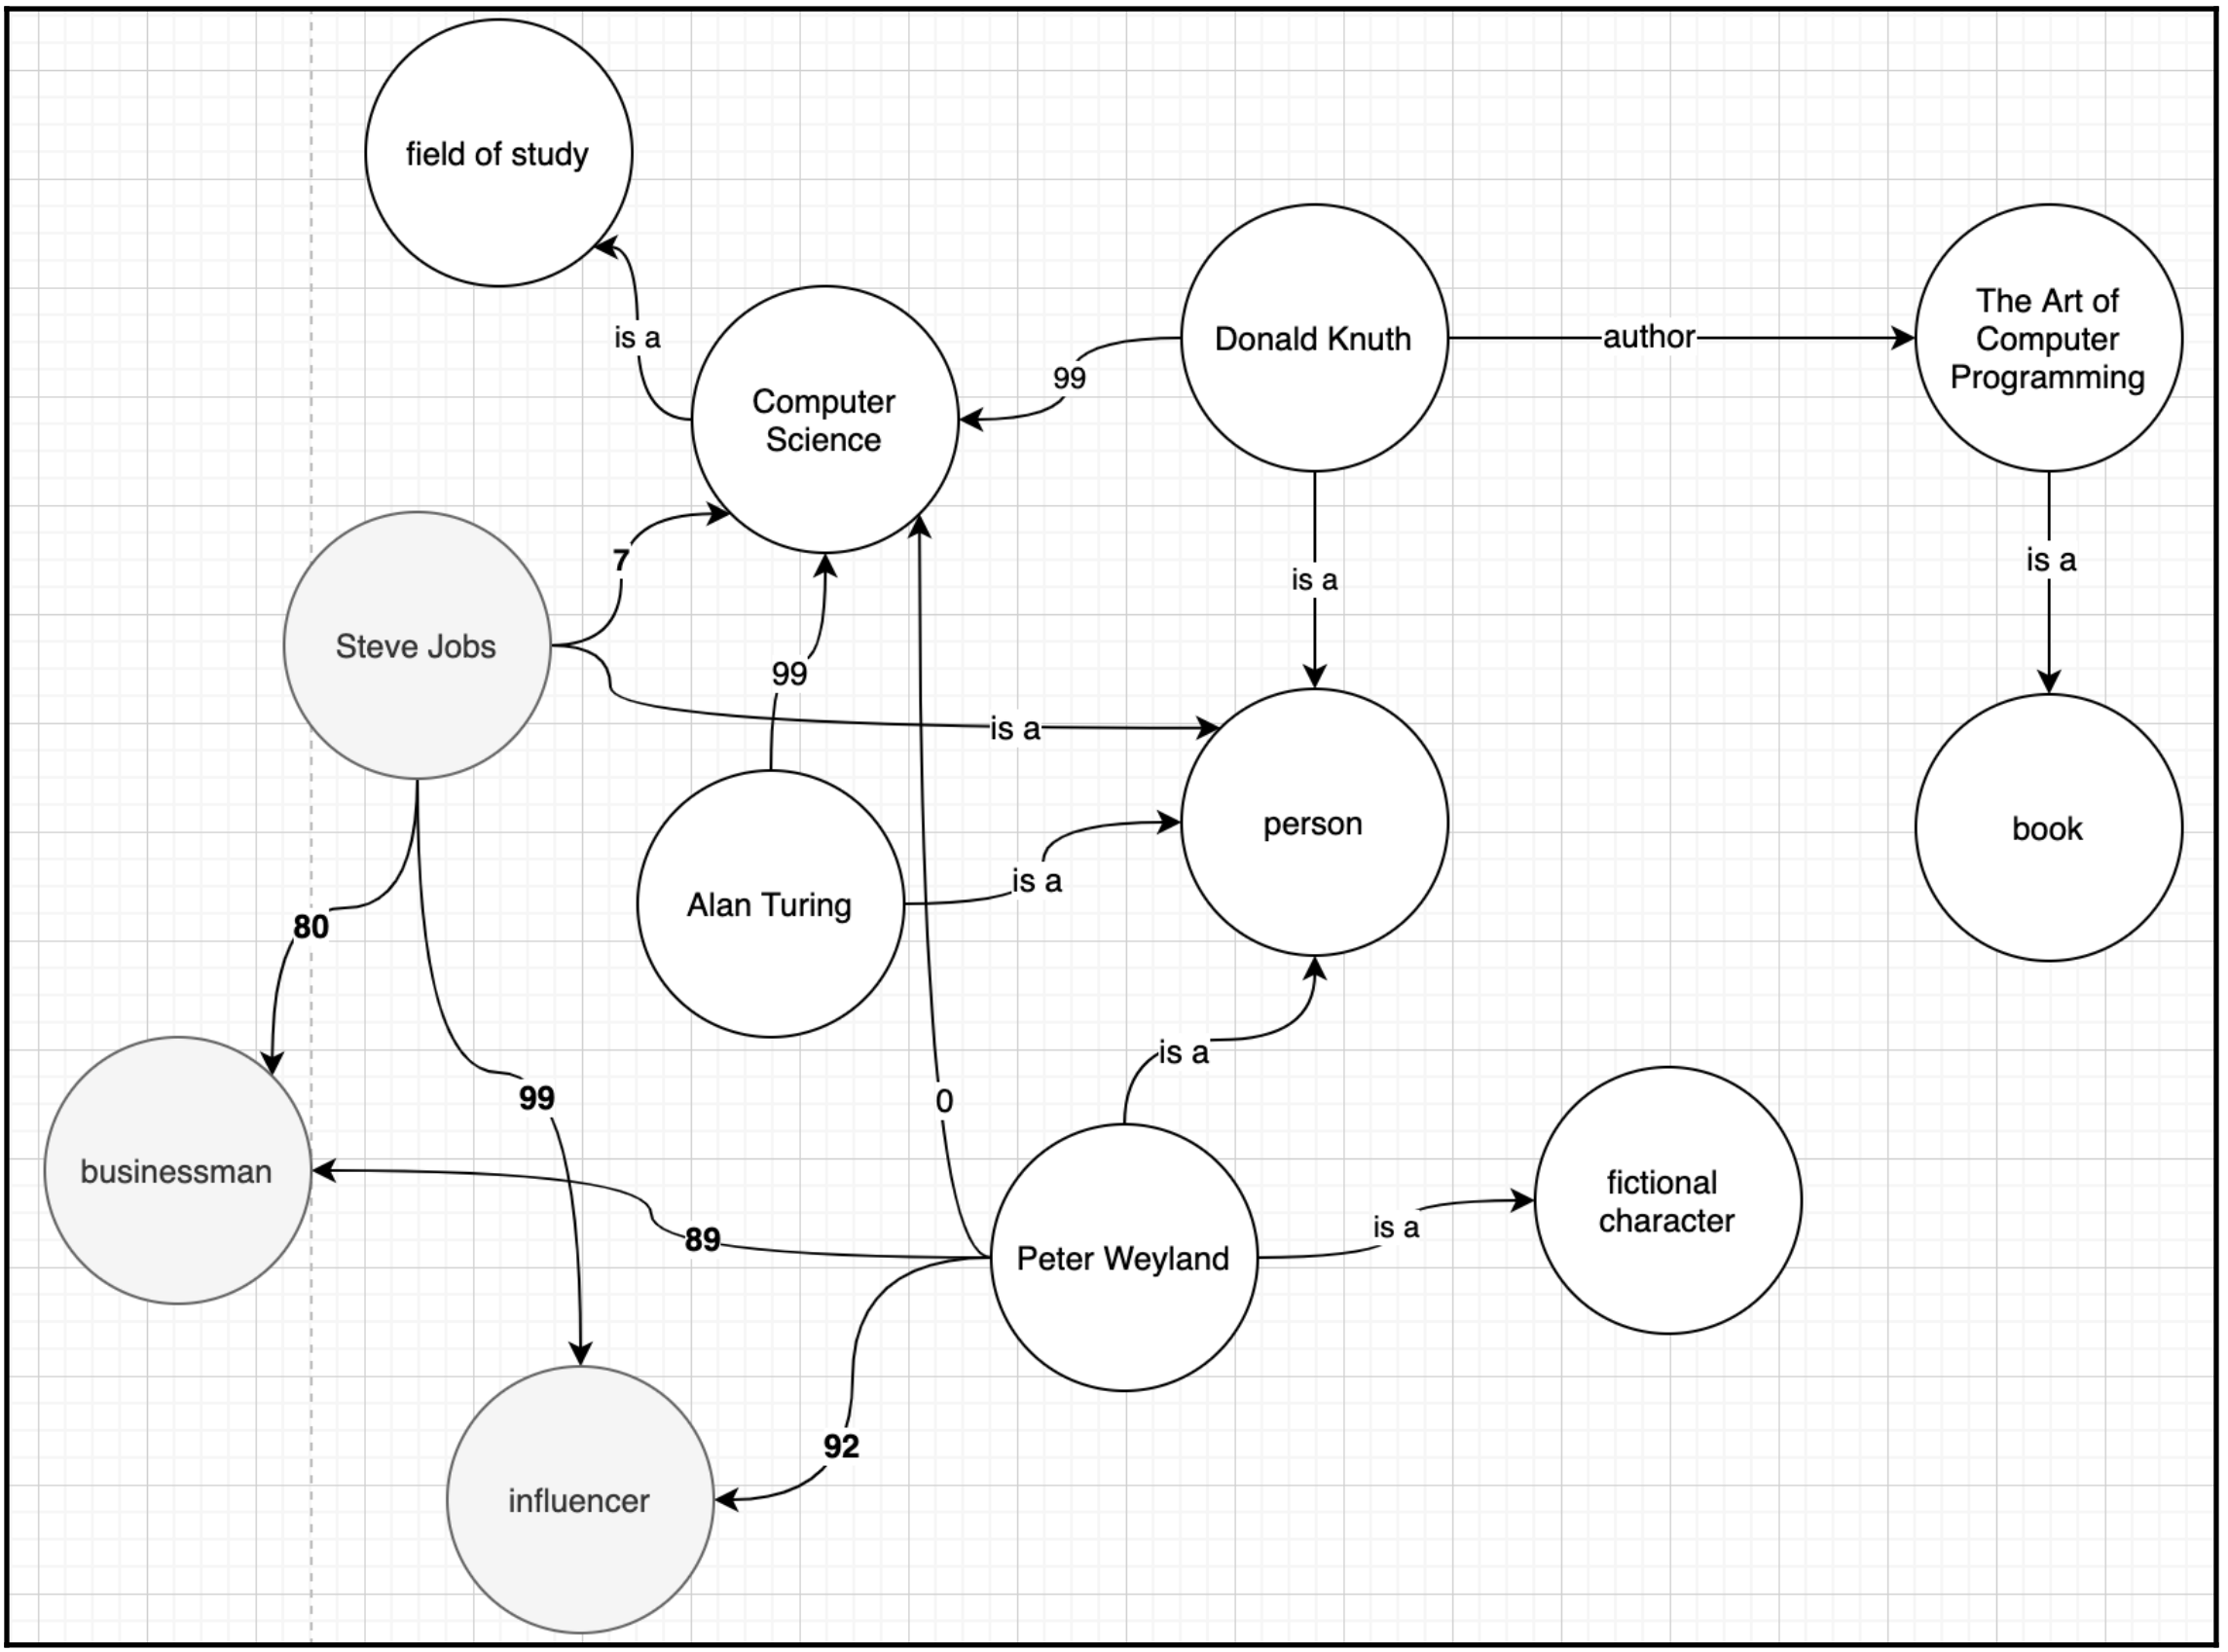
\includegraphics[width=0.8\textwidth]{content/Section-3/Chapter-16/16}
\end{center}

看看这些边的权值。Steve·Jobs与计算机科学有某种联系,但他主要与商人和有影响力的节点有关。同样,我们现在可以看到,Peter·Weyland与Steve·Jobs的共同点多于Donald·Knuth。现在,推荐引擎建议搜索Donald Knuth的用户也应该看看Alan·Turing,因为他们都是人和计算机科学相关,权重相等或接近相等。这是一个将这样的图表整合到搜索引擎中的很好的例子。接下来,我们将向您介绍如何使用类似的知识图来构建一个更智能的框架,以提供相关的搜索结果。我们称之为基于对话框的搜索。 \par

\noindent\textbf{}\ \par
\textbf{实现基于对话框的搜索引擎} \ \par
最后,让我们着手设计搜索引擎的一部分,它将为我们提供细粒度的用户界面。正如我们在本章开头提到的,基于对话框的搜索引擎涉及到构建一个用户界面,向用户询问与他们的查询相关的问题。这种方法最适用于结果不明确的情况。例如,搜索Donald的用户可能想到以下情况之一: \par

\begin{itemize}
	\item \textit{Donald Knuth}, 伟大的计算机科学家
	\item \textit{Donald Duck}, 卡通人物
	\item \textit{Donald Dunn}, 真实姓名是杰瑞德·邓恩,虚构人物
	\item \textit{Donald Trump}, 商人和美国第45任总统
\end{itemize}

前面的列表只是Donald搜索词潜在结果的一个小示例。那么,缺少基于对话的搜索引擎会做什么呢?它们为用户输入提供最佳匹配的相关结果列表。例如,在我写这本书的时候,搜索Donald的结果是一系列与Donald Trump有关的网站,尽管我脑子里想的是Donald Knuth。这里,我们可以看到用户的最佳匹配和最佳匹配之间的关系。 \par
搜索引擎收集了大量的数据用于个性化的搜索结果。如果用户在网站开发领域工作,他们的大多数搜索请求将以某种方式与该特定领域相关。这对于为用户提供更好的搜索结果非常有帮助,例如:用户有一个很大的搜索历史,主要包括与网站开发相关的请求,当搜索zepelin时,会得到更好、更集中的结果。理想的搜索引擎将提供到Zeplin应用程序的网站链接,以构建Web UI,而对于其他用户,该引擎将提供关于名为Led Zeppelin的摇滚乐队的信息。 \par
设计一个基于对话框的搜索引擎是为用户提供更好界面的下一步。现在,如果我们已经有了一个强大的知识库,构建它就足够简单了。我们将使用上一节中描述的知识图的概念。让我们假设当用户输入一个搜索词时,我们从知识图中获取所有匹配的主题,并得到用户的潜在搜索列表,如下图所示: \par

\begin{center}
	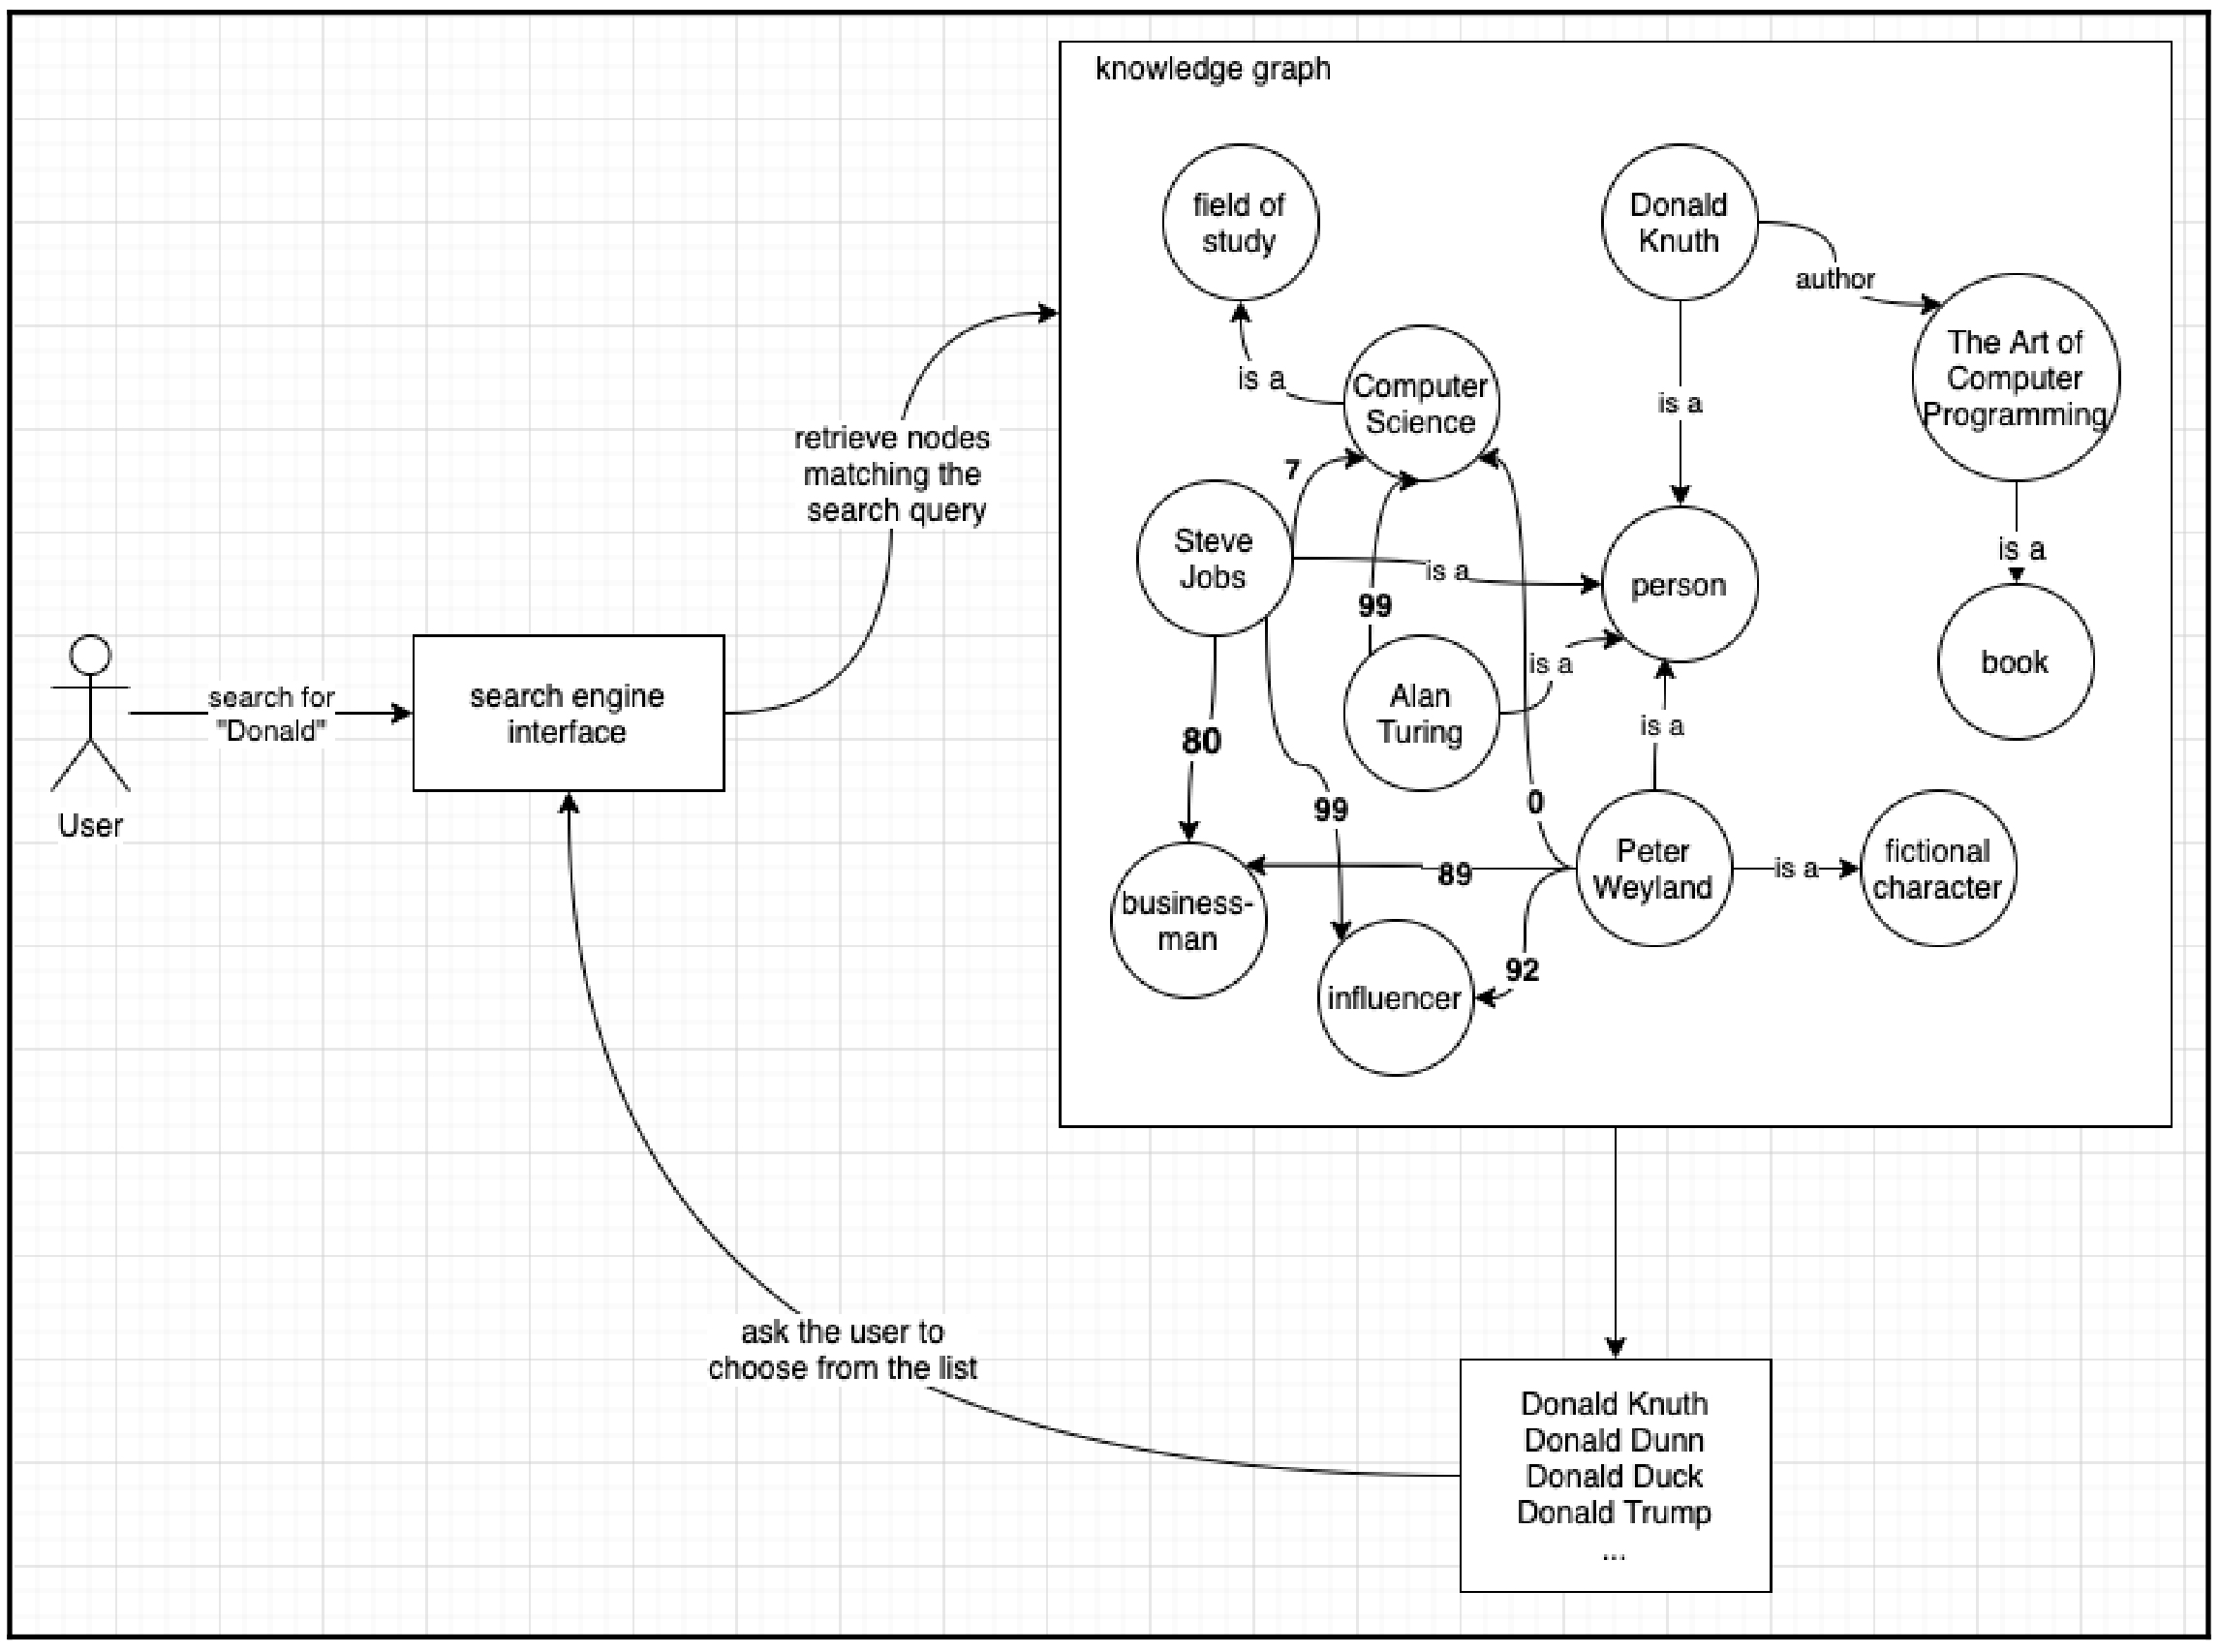
\includegraphics[width=0.8\textwidth]{content/Section-3/Chapter-16/17}
\end{center}

现在用户可以更容易地选择一个主题,并节省回忆全名的时间。当用户输入查询时,来自知识图的信息可以(对于某些搜索引擎来说是)并入自动建议中。此外,我们将处理搜索引擎的主要组成部分。显然,本章不能涵盖实现的每个方面,但我们将讨论的基本组件足以让你跳进自己的搜索引擎的设计和实现。 \par
我们不考虑搜索引擎的UI部分。我们最关心的是后台。当谈到应用程序的后端时,我们通常指的是用户不可见的部分。更具体地说,来看看下面的图表: \par

\begin{center}
	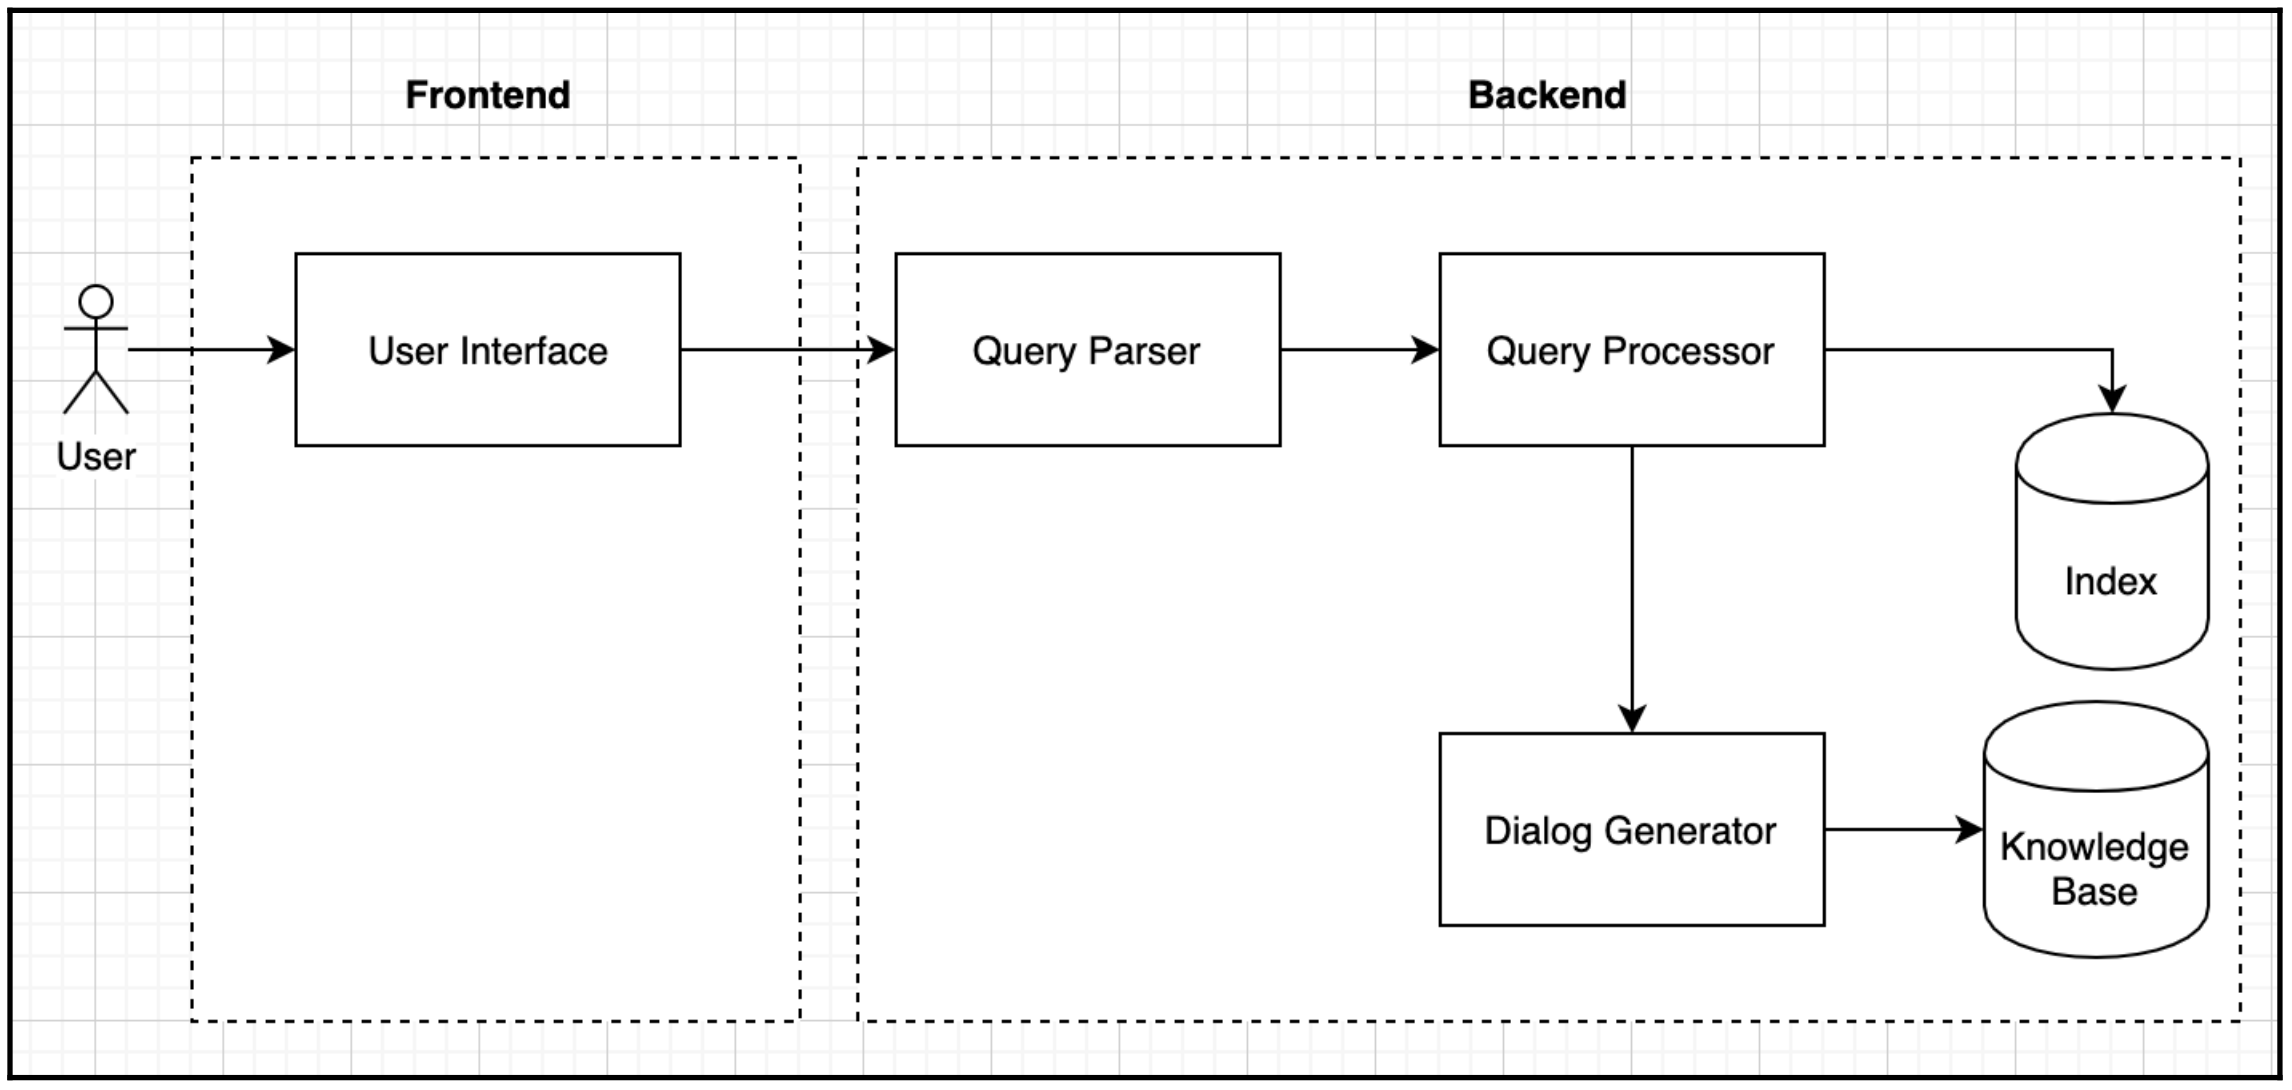
\includegraphics[width=0.8\textwidth]{content/Section-3/Chapter-16/18}
\end{center}

大部分引擎位于后端。虽然UI看起来很简单,但它是整个搜索系统的重要组成部分。这是用户开始他们的旅程的地方,用户界面越多的被设计来提供最好的可能的体验,当用户搜索时,不舒服的体验就越少。我们将专注于后端,下面是我们将要讨论的几个主要模块: \par

\begin{itemize}
	\item 查询解析器:分析用户查询、规范化单词,并收集查询中每个词汇的信息,以便稍后传递给查询处理器。
	\item 查询处理器:使用索引和补充数据库检索与查询关联的数据,并进行响应。
	\item 对话生成器:提供更多的选项供用户在搜索时选择。对话框生成器是一个补充模块。发出请求的用户可以省略这个对话框,或者使用它进一步缩小搜索结果的范围。
\end{itemize}

我们跳过了一些在搜索引擎中很常见的组件(比如爬虫),我们将把重点放在那些与基于对话框的搜索引擎密切相关的组件上。现在让我们从查询解析器开始。 \par

\noindent\textbf{}\ \par
\textbf{实现查询解析器} \ \par
查询解析器如其名称所示:解析查询。作为查询解析器的基本任务,我们应该用空格分隔单词。例如,用户查询zeplin best album会分为以下几个术语:zeplin、best和album。下面的类表示基本的查询解析器: \par

\begin{lstlisting}[caption={}]
// The Query and Token will be defined in the next snippet
class QueryParser
{
public:
	static Query parse(const std::string& query_string) {
		auto tokens = QueryParser::tokenize(query_string);
		// construct the Query object and return
		// see next snippet for details
	}

private:
	static std::vector<Token> tokenize(const std::string& raw_query) {
		// return tokenized query string
	}
};
\end{lstlisting}

看一下前面的parse()函数。它是这个类中唯一的公共函数。我们将添加从parse()函数调用的更多私有函数,以完全解析查询并作为查询对象获取结果。Query表示一个简单的结构体,包含关于查询的信息,如下所示: \par

\begin{lstlisting}[caption={}]
struct Query
{
	std::string raw_query;
	std::string normalized_query;
	std::vector<Token> tokens;
	std::string dialog_id; // we will use this in Dialog Generator
};
\end{lstlisting}

raw\underline{ }query是用户输入的查询的文本表示,normalized\underline{ }query是规范化后的相同查询。例如,如果用户输入了\texttt{good books, a programmer should read.}, \underline{ }query是精确的文本,normalized\underline{ }query是\texttt{good books programmer should read}。在下面的代码片段中,我们不使用normalized\underline{ }query,但在完成实现后,您将需要它。我们还将符号存储在Token的vector中,Token是一个结构体,如下所示: \par

\begin{lstlisting}[caption={}]
struct Token
{
	using Word = std::string;
	using Weight = int;
	Word value;
	std::unordered_map<Word, Weight> related;
};
\end{lstlisting}

相关属性表示与该标记语义相关的单词列表。如果两个词在概念上表达的意思相似,我们称之为语义相关的词。例如,“best”和“good”或者“album”和“collection”可以认为是语义相关的。您可能已经猜到了哈希表值中权重的用途,我们用它来存储相似度的权重。\par

\hspace*{\fill} \\ %插入空行

\includegraphics[width=0.05\textwidth]{images/warn}
权重的范围应该在使用搜索引擎时进行配置。假设我们选择的范围是0到99。best和good两个词的相似度权重可以用接近90的数字表示,而album和collection两个词的相似度权重可以在40 ~ 70之间偏离。选择这些数字是很棘手的,它们应该在引擎的开发和开发过程中进行调整。 \par
\noindent\textbf{}\ \par

最后,如果用户选择了生成器建议的路径,查询结构的dialog\underline{ }id表示生成的对话框的ID。我们很快就会讲到这个问题。现在让我们继续结束parse()函数。 \par
在QueryParser类添加的以下内容: \par

\begin{lstlisting}[caption={}]
class QueryParser
{
	public:
	static Query parse(const std::string& query_string,
	const std::string& dialog_id = "")
	{
		Query qr;
		qr.raw_query = query_string;
		qr.dialog_id = dialog_id;
		qr.tokens = QueryParser::tokenize(query_string);
		QueryParser::retrieve_word_relations(qr.tokens);
		return qr;
	}
private:
	static std::vector<Token> tokenize(const std::string& raw_string) {
		// 1. split raw_string by space
		// 2. construct for each word a Token
		// 3. return the list of tokens
	}
	static void retrieve_word_relations(std::vector<Token>& tokens) {
		// for each token, request the Knowledge Base
		// to retrieve relations and update tokens list
	}
};
\end{lstlisting}

虽然在前面的代码片段中没有实现两个私有函数(tokenize和retrieve\underline{ }word\underline{ }relations),但基本思想是它们对搜索查询进行规范化和收集信息。在实现查询处理器之前,先看一下前面的代码。 \par

\noindent\textbf{}\ \par
\textbf{实现查询处理器} \ \par
查询处理器完成搜索引擎的主要工作,从搜索索引中检索结果,并根据搜索查询响应一个相关的文档列表。在本节中,我们还将介绍对话框的生成。 \par
正如在前一节中看到的,查询解析器构造了一个包含令牌和dialog\underline{ }id的查询对象。我们将在这里的查询处理程序中使用这两种方法。 \par

\hspace*{\fill} \\ %插入空行

\includegraphics[width=0.05\textwidth]{images/tip}
考虑到可伸缩性,建议为对话框生成器使用单独的组件。出于学习目的,我们将保持实现的简洁,但您可以自由地重新设计基于对话框的搜索引擎,并完成实现以及爬虫和其他补充模块。 \par
\noindent\textbf{}\ \par

查询对象中的标记用于向搜索索引发出请求,以便检索与每个单词相关联的一组文档。下面是相应的QueryProcessor类的样子: \par

\begin{lstlisting}[caption={}]
struct Document {
	// consider this
};
class QueryProcessor
{
public:
	using Documents = std::vector<Document>;
	static Documents process_query(const Query& query) {
		if (!query.dialog_id.empty()) {
			// request the knowledge graph for new terms
		}
		// retrieve documents from the index
		// sort and return documents
	}
};
\end{lstlisting}

请将前面的代码片段视为对实现的介绍。我们想表达QueryProcessor类的基本思想。它有process\underline{ }query()函数,该函数根据query参数中的标记从索引中检索文档。这里的关键角色是搜索索引。就进行快速查询而言,定义其构造的方式和存储文档的方式是必不可少的。同时,作为附加参数提供的对话框ID允许process\underline{ }query()函数请求知识库(或知识图谱)来检索与查询相关的更多相关标记。 \par
同样重要的是,考虑到QueryProcessor还负责生成对话框(即定义一组路径,为用户提供查询的可能场景)。生成的对话框被发送给用户,当用户进行另一个查询时,使用的对话框将通过我们已经看到的对话框ID与该查询关联。 \par
虽然前面的实现主要是介绍性的(因为代码太大,不适合本章),但它进一步设计和实现引擎的基础。 \par

\noindent\textbf{}\ \par
\textbf{总结} \ \par
对于经验丰富的程序员来说,从零开始构建搜索引擎也是一项艰巨的任务。我们在这本书中涉及了很多话题,并在本章中通过设计一个搜索引擎将它们中的大部分结合起来。 \par
我们已经了解到,Web搜索引擎是由几个组件组成的复杂系统,如爬虫、索引器和用户界面。爬虫程序负责定期检查网页,下载网页给搜索引擎索引。索引导致了被称为倒排索引的大数据结构的产生。倒排索引,或者仅仅是索引,是一种数据结构,它将单词映射到它们所在的文档中。 \par
接下来,我们定义了什么是推荐引擎,并尝试为我们的搜索引擎设计一个简单的推荐引擎。推荐引擎与本章讨论的基于对话框的搜索引擎特性相连接。基于对话框的搜索引擎旨在向用户提供有针对性的问题,以了解更多关于用户实际想要搜索的内容。 \par
本书的最后,我们从C++的角度讨论了计算机科学的各种主题。从C++程序的细节开始,然后简要地讨论了使用数据结构和算法有效地解决问题。掌握一门编程语言并不足以在编程方面取得成功。而且,需要解决在数据结构、算法、多线程等方面需要大量技能的编码问题。此外,处理不同的编程范式可以改变对计算机科学的看法,并允许以全新的视角来解决问题。本书中,我们已经接触了几种编程范式,如函数式编程。 \par
最后,软件开发不仅仅局限于编码。构建和设计项目是成功应用程序开发的关键步骤之一。第10章到第16章,主要是关于设计现实世界应用程序的方法和策略。让这本书成为你以C++开发人员的角度了解编程世界的入门指南。通过开发更复杂的应用程序来提高你的技能,并与同事和那些刚刚开始职业生涯的人分享知识。 \par

\noindent\textbf{}\ \par
\textbf{问题} \ \par
\begin{enumerate}
	\item 爬虫程序在搜索引擎中的角色是什么?
	\item 为什么我们称搜索索引为反向索引?
	\item 在索引单词之前对单词进行标记的主要规则是什么?
	\item 推荐引擎的作用是什么?
	\item 什么是知识图谱?
\end{enumerate}

\noindent\textbf{}\ \par
\textbf{扩展阅读} \ \par
更多信息,请参阅以下书籍: \par
\begin{itemize}
	\item Introduction to Information Retrieval, Christopher Manning, et al., \\ https:/​/​www.​amazon.​com/Introduction-​Information-​Retrieval-​Christopher-​Manning/​dp/​0521865719/​
\end{itemize}

\newpage

































